\documentclass[../xlapes02]{subfiles}
\begin{document}
    \chapter{Reinforcement Learning}\label{ch:reinforcement-learning}

    The motivation for this chapter comes from the influential book on reinforcement learning by Richard Sutton and Andrew Barto and Foundations of Reinforcement Learning with Application in Finance by Ashwin Rao and Tikhon Jelvis~\cite{rao2022foundations, sutton2018reinforcement}.

    This chapter explores the application of Reinforcement Learning techniques in the context of portfolio allocation. In \cref{sec:markov-theory} we will provide an introduction to Markov models, first explore \emph{Markov Processes}, \emph{Markov Reward Processes} and \emph{Markov Decision Processes}, which are the fundamental building blocks of Reinforcement Learning. Afterward, we divide Reinforcement Learning into two main categories. In \cref{sec:model-based-methods}, we will discuss \emph{Model-based} Reinforcement Learning methods, and in \cref{sec:model-free-methods} we will discuss \emph{Model-free} Reinforcement Learning methods in detail with advantages and disadvantages of each approach. Let's start with an introduction to AI in general and its different types of learning:

    \paragraph{Supervised Learning}
    In supervised learning (SL), a model is trained on a labeled dataset, where the input data is paired with corresponding output labels. The model learns to make predictions based on the labeled examples, and the goal is to minimize the error between predicted outputs and actual labels. Common applications of supervised learning include image classification, speech recognition, and sentiment analysis.

    \paragraph{Semi-supervised Learning}
    Semi-supervised learning (SSL) is a combination of supervised and unsupervised learning. It uses a small labeled dataset along with a large unlabeled dataset for training. The model leverages the limited labeled examples to learn patterns from the unlabeled data and then makes predictions on unseen data. SSL is useful when obtaining labeled data is expensive or time-consuming. It is often used in scenarios where obtaining a large labeled dataset is challenging, such as in medical diagnosis or fraud detection.

    \paragraph{Unsupervised Learning}
    In unsupervised learning (UL), the model learns from unlabeled data without any predefined output labels. The goal is to find underlying patterns, structures, or relationships within the data. Everyday unsupervised learning tasks include clustering, dimensional reduction, and anomaly detection. UL is used in scenarios where labeled data is scarce or not available, and the model needs to discover patterns autonomously from the data.

    The last type is Reinforcement Learning and this entire chapter will be devoted to it, let's dive into it in more detail.


    \section{Introduction}\label{sec:rl-introduction}
    Reinforcement learning (RL) is an exciting field at the intersection of artificial intelligence (AI) and machine learning (ML) that deals with training agents to make optimal decisions in dynamic environments. RL is inspired by the way humans learn from experience, like \texttt{trial-and-error}, and an agent interacts with an environment the same way and receives feedback in the form of \emph{rewards} (typically positive number, e.g.: $1$) or \emph{penalties} (typically negative number, e.g.: $-1$), and uses this feedback to learn and improve its decision-making abilities.

    At the heart of RL lies the concept of an agent, which takes actions in an environment to achieve specific goals. The environment is typically modeled as a Markov decision process (MDP), later defined in \cref{subsec:markov-decision-process}, which is a mathematical framework that describes how an agent interacts with an environment in discrete time steps.
%    An MDP is defined by a tuple $(S, A, P, R)$, where $S$ is the state space, $A$ is the action space, $P$ is the transition probability function, and $R\in\mathbb{R}$ is the reward.

    The goal of an RL agent is to learn a policy, denoted by $\pi$, which is a mapping from states to actions that maximize the cumulative reward $G_t$ over time $T$. The agent uses this policy to select actions at each time step, and the environment responds with a new state and a reward. The agent then updates its policy based on the observed rewards and states, aiming to improve its decision-making abilities and achieve higher rewards in the long run. This is the RL advantage because, unlike supervised learning, RL does not require labeled data~\cite{rl-course-david-silver}.

%    RL algorithms can be broadly categorized into two main types: model-free and model-based. Model-free algorithms are then further divided into value-based and policy-based methods, such as Q-learning (value-based) and policy gradient methods (policy-based), which learn directly from the interactions with the environment without explicitly modeling the transition probabilities and rewards. Model-based algorithms, on the other hand, learn a model of the environment and use it to make decisions. These algorithms have their strengths and weaknesses, and the choice between them depends on the specific problem and requirements.

    The sequence of states, actions, and rewards that the agent experiences is called a trajectory, and it looks like this:
    \begin{equation}
        \label{eq:trajectory}
        (S_0, A_0, R_1, S_1, A_1, R_2, S_2, A_2, \dots, S_{T-1}, A_{T-1}, R_T, S_T)
    \end{equation}

    This sequence of \emph{state-action-reward} can be finite or infinite, depending on the environment and the agent's goal. A pretty good example of this is the game of chess, where the game ends when one of the players wins or the game is a draw. In this case, the trajectory is finite, and the agent's goal is to maximize the cumulative reward over time $T$. On the other hand, the self-driving car example is an infinite-horizon problem, where the agent's goal is to maximize the cumulative reward over an infinite time horizon or until the car reaches its destination~\cite{FITMT25127}.

    \begin{figure}[h]
        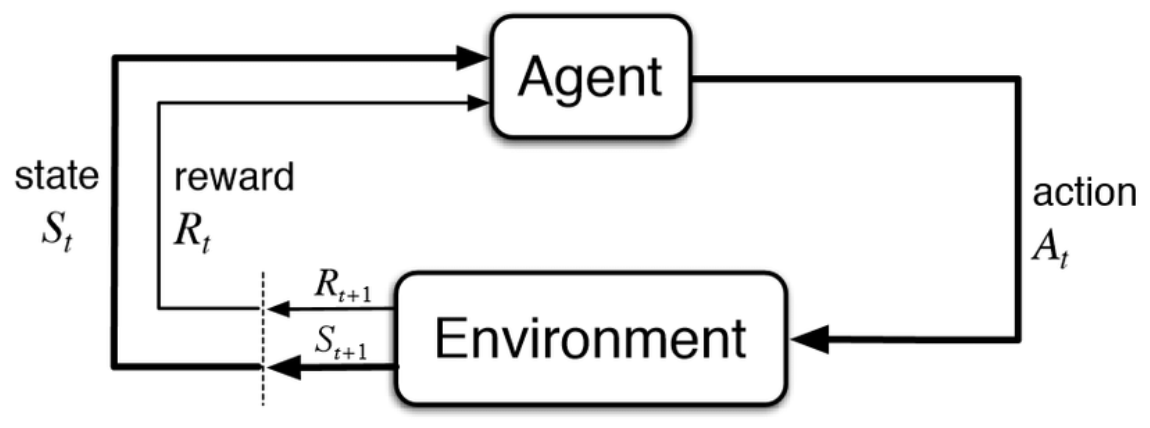
\includegraphics[width=0.7\linewidth]{image/agent-environment}
        \centering
        \caption{The agent interacts with the environment and learns to maximize the cumulative reward over time $T$.}
        \label{fig:rl-introduction}
    \end{figure}

    Because RL algorithms are categorized by the way it learns, there are many different types of RL algorithms. Based on the different approaches we can categorize RL algorithms into these clasess:
    \begin{multicols}{2}
        \begin{itemize}
            \item \textbf{Value-based}
            \begin{itemize}
                \item \textcolor{darkgray}{No Policy (implicit)}
                \item Value function
            \end{itemize}
            \item \textbf{Policy-based}
            \begin{itemize}
                \item Policy
                \item \textcolor{darkgray}{No Value function}
            \end{itemize}
            \item \textbf{Actor-critic}
            \begin{itemize}
                \item Policy
                \item Value function
            \end{itemize}
        \end{itemize}
        \columnbreak
        \begin{itemize}
            \item \textbf{Model-based}
            \begin{itemize}
                \item Policy and/or Value function
                \item Model
            \end{itemize}
            \item \textbf{Model-free}
            \begin{itemize}
                \item Policy and/or Value function
                \item \textcolor{darkgray}{No model}
            \end{itemize}
        \end{itemize}
    \end{multicols}

    As we can see in \cref{fig:model-value-policy-introduction}, the main difference is that the agent/algorithm learns the decision process based on \emph{Value-based methods}, \emph{Policy-based methods}, \emph{Model-based models} or some other combination of these classes. In this section, we explain the concepts of \emph{Value-based methods} in \cref{sec:value-based-learning} and \emph{Policy-based methods} in \cref{sec:policy-based}, and leave untouched \emph{Model-based methods} as this work does not use them in the implementation.

%    \emph{Model-based} algorithms are closely related to \emph{Planning algorithms} which are trying to create a model of the environment and use it to make decisions, they have knowledge of the transition probabilities and rewards from the beginning, we will discuss them in \cref{sec:model-based-methods}. \emph{Value-based} algorithms can implicitly infer a policy, but do not explicitly compute it, we will discuss them in \cref{sec:value-based-methods}, and \emph{Policy-based} algorithms compute a policy function by themselves, and are discussed in \cref{sec:policy-based-methods}. Another agent like \emph{Actor-critic methods} compute a policy function and a state-value function at the same time~\cite{rl-course-david-silver, sutton2018reinforcement}.

    \begin{figure}[h]
        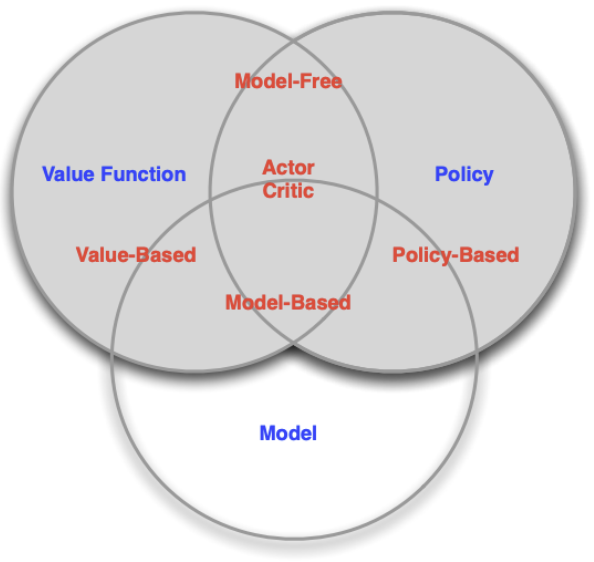
\includegraphics[width=0.5\linewidth]{image/model-value-policy}
        \centering
        \caption{The relationship between model, value function and policy. Source:~\cite{FITMT25127}}
        \label{fig:model-value-policy-introduction}
    \end{figure}


    \section{Markov Theory}\label{sec:markov-models-for-rl}
    This section provides an introduction to Markov theory, which is the fundamental building block of Reinforcement Learning. We begin by \emph{Markov Process}, described in~\cref{subsec:markov-process}, which is a stochastic process that satisfies the Markov property. We then move on to \emph{Markov Reward Process}, described in~\cref{subsubsec:markov-reward-process}, which is a Markov process with a reward function. Finally, we describe the most important for RL \emph{Markov Decision Process}, described in~\cref{subsec:markov-decision-process}, which is a Markov Reward process with decision-making ability.

    \subsection{Markov Process}\label{subsec:markov-process}
    The Markov process (MP), also known as Markov Chains, describes the states of an environment and models the dynamics of state transitions. In an MP, an agent can only observe the changing states of the environment and has no influence over them. Markov process has two key properties. Firstly, state transitions are non-deterministic. States are modeled as realizations of random variables, defined in \cref{subsubsec:probability-functions}. Secondly, the future state is only dependent on the current state, and not on previous states, simplifying causality with the Markov property~\cite{rao2022foundations, inproceedings}.

    \subsubsection{Probability Functions}\label{subsubsec:probability-functions}
    The first property of an MP states that each concrete state of an environment is the realization of a discrete random variable $X$ from set $V$ with a certain probability $Pr\left[X=x\right]$, where $x \in V$ and set $V$ contains all states of an environment. A state is a realization of a random experiment that the environment assumes with a certain probability, and this can be represented as a probability function~\cite{FITMT25127}:
    \begin{equation}
        P(X = X(\omega)) = P(X = x)
    \end{equation}

    The repeated successive execution of a random experiment can be represented as a stochastic process, which is a sequence of random variables, e.g., $X_t(\omega), X_{t+1}(\omega), \ldots X_n(\omega)$, where a single term can be shortened to $X_t$ and it represents the state of the environment at time $t$, $t\in\mathbb{N}$, $\omega$ is an elementary outcome of all possible outcomes $\Omega$~\cite{inproceedings, rao2022foundations}.

    \subsubsection{Stochastic Process (Random Process)}\label{subsubsec:stochastic-process}
    A stochastic process is defined as a collection of random variables defined on a common probability space $(\Omega, \mathcal{F}, P)$, where $\Omega$ is a sample space, $\mathcal{F}$ is a $\sigma$-algebra, and $P$ is a probability measure, and the random variables, indexed by some set $T$, all take values in the same mathematical space $S$, which must be measurable with respect to some $\sigma$-algebra $\Sigma$. In other words, stochastic process is a collection of random variables $X_t$, indexed by time $t$, so definition is~\cite{enwiki:1148510872}:
    \begin{equation}
        X_0, X_1, X_2,\cdots \text{ for discrete-time}
    \end{equation}
    or
    \begin{equation}
        \{X_t\}_{t\geq0} \text{ for continuous-time.}
    \end{equation}

    In stochastic processes the probability that the environment assumes a certain state depends on the realized states of previous random variables. For example, if the weather forecast is assumed to be a stochastic process, then yesterday’s weather may still have an influence on tomorrow’s weather. To represent this causality complicates the modeling of stochastic processes so that with the definition of Markov property, in \cref{subsubsec:markov-property}, the dependence of future states is assumed only on the current state. This is the second important property of the Markov process~\cite{FITMT25127}.

    \subsubsection{Markov Property}\label{subsubsec:markov-property}
    The Markov property, which is defined using conditional probability, states that ``The future is independent of the past, given the present."

    The stochastic process has the Markov property if and only if, for all time steps $t \in I$, where $I$ is some (totally ordered) set, the conditional probability of the next state given the current state is equal to the conditional probability of the next state given all the previous states: $Pr\left[X_{t+1}|X_t\right] = Pr\left[X_{t+1}|X_1,\ldots,X_t\right]$

    This property has several advantages in practical reinforcement learning, including the uniqueness and distinctiveness of states, as well as the ability to precisely formulate the probability of state transitions, defined as:~\cite{FITMT25127}
    \begin{equation}
        \mathcal{P}(x'|x)=Pr\left[X_{t+1}=x'|X_t=x\right]
    \end{equation}

    Given $n$ possible states, $s\in \mathcal{S}$, then the probability of transitioning from state $s$ to state $s'$ can be represented as a matrix $\mathcal{P}$, and because probability summation rule, the sum of transition probabilities from state $s$ to any other state $s'$ must equal to $1$.

    \begin{definition}
        The Markov process is a stochastic process that satisfies the Markov property and is described as tuple $\left(\mathcal{S}, \mathcal{P}\right)$ for which holds:\cite{ABATE2021102207}
        \begin{itemize}
            \item $\mathcal{S}=s_1,s_2,\cdots,s_n$ is a finite set of states
            \item $\mathcal{P}$ is an $n\times n$ transition probability matrix which sums to 1 for each row, so each value $p_{ij}$ is the probability of transitioning from state $s_i$ to state $s_j$ in interval $\left< 0;1 \right>$
        \end{itemize}
    \end{definition}

    \begin{align*}
        \mathcal{P}=\begin{bmatrix}
                        p_{11} & p_{12} & p_{13} & \dots  & p_{1n} \\
                        p_{21} & p_{22} & p_{23} & \dots  & p_{2n} \\
                        \vdots & \vdots & \vdots & \ddots & \vdots \\
                        p_{n1} & p_{n2} & p_{n3} & \dots  & p_{nn}
        \end{bmatrix}
    \end{align*}

    \subsubsection{Starting States}
    The probability distribution of start states is denoted as $\mu : N \rightarrow [0,1]$ in order to perform simulations and compute the probability distribution of states at specific future time steps. A Markov Process is fully specified by the transition probability function $\mathcal{P}$, which governs the complete dynamics of the process.
    \begin{itemize}
        \item Specification of the transition probability function $\mathcal{P}$.
        \item Specification of the probability distribution of start states (denote this as $\mu : N \in[0, 1])$.
    \end{itemize}
    Given $\mu$ and $\mathcal{P}$, we can generate sampling traces of the Markov Process and answer questions such as the probability distribution of states at specific future time steps or the expected time of the first occurrence of a specific state, given a certain starting probability distribution $\mu$. The separation of concerns between $\mathcal{P}$ and $\mu$ is key to the conceptualization of Markov Processes~\cite{rao2022foundations}.

    \subsubsection{Terminal States}
    Markov Processes can terminate at specific state (e.g., based on rules for winning or losing in games). Termination can occur after a variable number of time steps (episodic) or after a fixed number of time steps (as in many financial applications). If all sampling traces of the Markov Process reach a terminal state, they are called episodic sequences. The notion of episodic sequences is important in Reinforcement Learning. In some financial applications, the Markov Process terminates after a fixed number of time steps $T$, and states with time index $t = T$ are labeled as terminal states. States with time index $t < T$ transition to states $S_{t+1}$ with time index $t + 1$~\cite{rao2022foundations}.

    \begin{figure}[h!]
        \begin{center}
            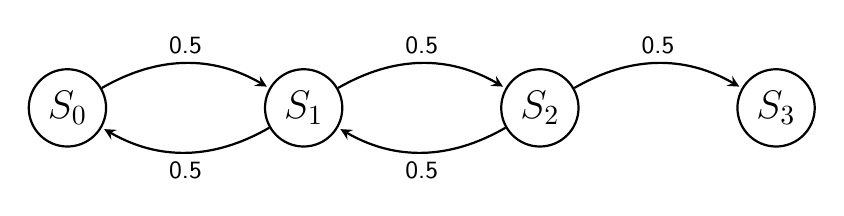
\begin{tikzpicture}
                [->,>=stealth,shorten >=1pt,auto,node distance=3cm,
                thick,main node/.style={circle,draw,font=\sffamily\Large\bfseries}]

                % Nodes
                \node[main node] (A) {$S_0$}; % Starting state
                \node[main node] (B) [right of=A] {$S_1$};
                \node[main node] (C) [right of=B] {$S_2$};
                \node[main node] (T) [right of=C] {$S_3$}; % Terminal state

                % Edges
                \path[every node/.style={font=\sffamily\small}]
                (A) edge [bend left] node [above] {0.5} (B)
                (B) edge [bend left] node [below] {0.5} (A)
                (B) edge [bend left] node [above] {0.5} (C)
                (C) edge [bend left] node [below] {0.5} (B)
                (C) edge [bend left] node [above] {0.5} (T);
            \end{tikzpicture}
            \caption{Markov Process with Start state $S_0$ and Terminal state $S_3$, because there is no edge from $S_3$.}
            \label{fig:markov-process}
        \end{center}
        \centering
    \end{figure}

    The examples shown here only include states and transition probabilities. To fully define an environment within the framework of RL, actions, and rewards also need to be defined, so in the next section, we will introduce Markov Reward Process (MRP) and Markov Decision Process (MDP) to be able to define RL environments~\cite{sutton2018reinforcement}.

    \subsection{Markov Reward Process}\label{subsubsec:markov-reward-process}
    Markov Reward Process (MRP) is a Markov Process with rewards. These rewards are random, and all we need to do is to specify the probability distributions of these rewards as we make state transitions. The main purpose of Markov Reward Processes is to calculate how much reward we would accumulate (in expectation, from each of the non-terminal states) if we let the process run indefinitely, bearing in mind that future rewards need to be discounted appropriately $\gamma$ (otherwise, the sum of rewards could blow up to $\infty$). In order to solve the problem of calculating expected accumulative rewards, defined in \cref{par:expected-reward}, from each non-terminal state, we will first set up some formalism for Markov Reward Processes and develop some theory on calculating rewards accumulation~\cite{rao2022foundations}.

    The main objective of an RL agent is to maximize the sum of rewards from each time step. The agent can observe different episodes in the Markov process but lacks the means to determine the actual quality of an episode. By calculating the reward, we can precisely measure the goodness of an episode or even a single state using the \emph{state-value function}, defined in \cref{subsubsec:state-value-function}. This allows the agent to actively transition to favorable states and maximize the reward~\cite{rao2022foundations}.

%    \begin{definition}
%        A Markov Reward Process is a Markov Process with a time-indexed sequence of Reward random variables $R_t \in D$ (a countable subset of $R$) for time steps $t = 1, 2, \cdot$, satisfying the Markov Property (including Rewards): $P[(Rt+1, St+1)|St, St−1, ..., S0] = P[(Rt+1, St+1)|St]$ for all $t ≥ 0$.
%    \end{definition}

    \begin{definition}
        \textbf{Markov Reward Process} is a Markov Process, along with a time-indexed sequence of Reward random variables $R_t \in D$ (a countable subset of $\mathbb{R}$) for time steps $t = 1, 2, \ldots$, satisfying the Markov Property (including Rewards): $\mathcal{P}(R_{t+1},S_{t+1})|S_t,S_{t-1}, \ldots, S_0] = P[(R_{t+1}, S_{t+1})|S_t]$ for all $t \geq 0$. MRP is a tuple $(\mathcal{S},\mathcal{P},\mathcal{R},\gamma)$ for which holds:\cite{rao2022foundations}
        \begin{itemize}
            \item $\mathcal{S}=s_1,s_2,\cdots,s_n$ is a finite set of states
            \item $\mathcal{P}$ is an $n\times n$ transition probability matrix which sums to 1 for each row, so each value $p_{ij}$ is the probability of transitioning from state $s_i$ to state $s_j$ in interval $\left< 0;1 \right>$
            \item $\mathcal{R}$ is a sequence of random variables $R_1,R_2,\cdots,R_n$ where $R_t$ is a random variable that represents the reward for transitioning from state $s_t$ to state $s_{t+1}$
            \item $\gamma$ is a discount factor in interval $\left<0;1\right>$
        \end{itemize}
        \begin{equation}
            \mathcal{P}(s,r,s')=Pr\left[R_{t+1}=r,S_{t+1}=s'|S_t=s\right]\text{ for time steps }t=0,1,2,\ldots
        \end{equation}
        \begin{align*}
            \text{ for all }s\in N,r\in D,s'\in S,\text{ such that }\sum_{s'\in S}\sum_{r\in D}\mathcal{P}(s,r,s')=1\text{ for all }s\in N
        \end{align*}
    \end{definition}

    \subsubsection{Reward function}\label{par:reward-function}
    The reward function $\mathcal{R}(s)$ is a function that maps a state $s$ to a reward $r$ and specifies how much reward and agent expects from the environment given current state $s$. If an agent is in a state $s$ at time $t$, the agent receives reward  $R_{t+1}$  at time $t + 1$,  when it transitions to a subsequent state $s'$. Rewards of an episode can be represented as a sequence $(R_1, R_2, \ldots, R_t)$~\cite{FITMT25127}.

    % TODO: Agent reference

    \paragraph{When to receive the reward?} An RL agent, defined in \verb|\cref{TODO}|, should receive a reward for a good action and a penalty for a bad action. Good actions are those that lead to the agent's main goal, while bad actions are those that lead to a state that is not desirable for the agent. That is, an agent should not receive (one small) reward when it can then receive a large penalty, for example in chess by taking one piece, when it can then lose the game by getting checkmate~\cite{sutton2018reinforcement}.

    \subsubsection{Expected reward}\label{par:expected-reward}
    The expected reward, denoted as $G_t$ at time $t$ is the discounted sum of rewards in a single episode, is defined as:
    \begin{equation}
        G_t=R_{t+1}+\gamma R_{t+2}+\gamma^2 R_{t+3}+\ldots=\sum_{k=0}^{\infty}\gamma^k R_{t+k+1}
    \end{equation}

    We can also calculate the expected rewards for state-action pairs as a two-argument function $r:S\times A\to R$, is defined as:
    \begin{equation}
        r(s,a)=\sum_{t=0}^{\infty}\gamma^t R_{t+1} P(S_{t+1}=s'|S_t=s,A_t=a)
    \end{equation}

    \paragraph{Discount factor $\gamma$}\label{par:discount-factor}
    The calculation also involves the discount factor $\gamma$ which is a value in the interval $\langle 0, 1 \rangle$. If $\gamma$ is equal to one, then the expected reward can goes to infinity, that is why the agent can only calculate the reward in the case of always terminating episodes. If $\gamma$ is less than one, the reward has a finite value, allowing the agent to determine the quality of an episode. The discount factor is not only useful mathematically but also for tuning the agent's rewards. If early rewards in an episode are more significant than later ones, $\gamma$ should be close to zero. If the rewards represent monetary gains, then it is the case, as early rewards earn additional interest. On the other hand, the closer $\gamma$ is to one, the more important later rewards are~\cite{rao2022foundations, sutton2018reinforcement, perotto:hal-02363599}.

    \subsubsection{State-value Function}\label{subsubsec:state-value-function}
    The state-value function provides information about the long-term expected reward for each state in an environment. With this information, an agent can determine which state to transition to in order to maximize the reward of an episode. Specifically, the agent should choose the state that has the highest long-term expected reward. If the agent observes a sequence of states and rewards, it can remember the subsequent rewards for each state, calculate the reward of an episode, and iteratively update the probabilities for a higher occurrence of rewards over multiple episodes. As the number of episodes approaches infinity, the estimated probabilities converge to the true probabilities, and the long-term expected reward of a state can be accurately determined. Intuitively, the more episodes and consequent rewards an agent observes, the better it can estimate the value of each state. We will introduce the methods for determining the state-value function and the action-value function in the next subsection, along with a recursive iterative approach for calculating the state-value function based on Bellman's equation~\cite{FITMT25127}.

    Since episodes may start with different states due to state transition probabilities, the expected reward of a particular state is the expected value of the conditional density function over the probabilities of rewards for that state. Thus, $G_t$ can be treated mathematically as a continuous random variable.
    To derive \emph{Bellman's equation}, defined later in this subsection, we need to make use of the definition of the \emph{(Recursive) State-value function}~\cite{FITMT25127, rao2022foundations}.
    \begin{equation}
        \label{eq:state-value-function}
        \begin{split}
            \textcolor[RGB]{50,150,50}{v(s)}&=E[G_t|S_t=s]\\
            &=E[R_{t+1}+\gamma G_{t+1}|S_t=s]\\
            &=E[R_{t+1}+\gamma\textcolor[RGB]{50,150,50}{v(S_{t+1})}|S_t=s]\\
            &=\mathcal{R}(s)+\gamma\sum_{s'\in\mathcal{S}}\mathcal{P}(s'|s)\textcolor[RGB]{50,150,50}{v(s')}
        \end{split}
    \end{equation}
    where $\gamma$ is the discount factor, $\mathcal{R}(s)$ is the immediate reward for state $s$, $\mathcal{P}(s'|s)$ is the transition probability from state $s$ to state $s'$, and $\mathcal{S}$ is the set of all possible states in the environment. The last equation expresses that the long-term expected reward of a state depends only on the immediate reward and the long-term expected reward of the subsequent states.

    In the case of Finite Markov Reward Processes, let's assume that the state space is denoted as $\mathcal{S} = \{s_1, s_2, ..., s_n\}$, and the subset of states of interest is denoted as $\mathcal{N}$ with $m \leq n$ states. We can use bold-face notation to represent functions as column vectors and matrices since we are dealing with finite states/transitions. So, $V$ is a column vector of length $m$, $P$ is an $m \times m$ matrix, and $R$ is a column vector of length $m$ (with rows/columns corresponding to states in $\mathcal{N}$). We can express the equation in vector and matrix notation as follows:
    \begin{equation}
        \begin{split}
            \bm{V}&=\bm{\mathcal{R}}+\gamma \bm{\mathcal{P}}\cdot \bm{V}\\
            &=(\bm{I_m}-\gamma \bm{\mathcal{P}})^{-1}\cdot \bm{\mathcal{R}}
        \end{split}
    \end{equation}
    where $\bm{I_m}$ is the identity matrix of size $m\times m$, and $\gamma$ is the discount factor~\cite{rao2022foundations}.

    By extending the \cref{subsubsec:state-value-function} to include actions, we arrive at the most important equation in all of the reinforcement learning: \emph{The Bellman equation}, defined in ~\cref{subsubsec:bellman-equation}. It states that to calculate the long-term expected reward from a state, an agent only needs to add together the reward of the current state and the long-term expected reward of the next state~\cite{FITMT25127}.

    \subsection{Markov Decision Process}\label{subsec:markov-decision-process}
    The Markov Decision Process (MDP) allows an agent to actively influence changes in the state of the environment through its actions. Within the MDP, the agent has the ability to jointly determine the subsequent state to which the environment should transition. The agent's primary goal is to strategically choose actions that maximize the expected payoff. In the previous subsections, we addressed the aspect of \emph{sequential uncertainty (e.g., MRP)} using the Markov process framework and extended it to include the uncertain reward $R_t\in\mathcal{R}$ at each state transition $p(s',r,s)$, referred to as Markov reward processes. However, this framework lacks the notion of \emph{sequential decision making} and in this section, this notion is introduced in terms of MDP, a generalization of MRP that includes the notion of \emph{sequential decision making}~\cite{rao2022foundations}.
%
    \begin{definition}
        \emph{Markov decision process} is the Markov reward process with actions. It is an tuple $(S,A,\mathcal{P},\mathcal{R},\gamma)$, where:
        \begin{itemize}
            \item $\mathcal{S}$ is finite set of states, known as the State Space
            \item $\mathcal{A}$ is finite set of actions, known as the Action Space
            \item $\mathcal{P}$ is a transition probability function $p(s',r,s,a)$, which is a function that maps a state $s$, an action $a$, a next state $s'$ and a reward $r$ to a probability $p(s',r,s,a)$
            \item $\mathcal{R}$ is a reward function $r(s,a)$, which is a function that maps a state $s$ and an action $a$ to a reward $r(s,a)$
            \item $\gamma\in[0,1]$ is the discount factor
        \end{itemize}
    \end{definition}

    \subsubsection{Stochastic Policy function}\label{subsubsec:policy}
    A Stochastic Policy function, denoted by $\pi$, in the context of MDPs, is a function that maps states to actions. It represents the agent's decision-making strategy for selecting actions based on the current state.
    \begin{definition}
        A policy is defined as $\pi: \mathcal{S} \rightarrow \mathcal{A}$, where $\mathcal{S}$ is the set of states and $\mathcal{A}$ is the set of actions. Notation for a policy is as follows:
        \begin{equation}
            \label{eq:policy}
            \pi(a|s)=\mathbb{P}(A_t=a|S_t=s)
        \end{equation}
    \end{definition}
    Policy refers to the specification of an Agent's actions based on the current state in a Markov Decision Process. The policy can be deterministic, meaning it selects a single action for each state. It is represented as a function $\pi_D : N \rightarrow \mathcal{A}$, where $\pi_D(s)$ represents the action to be taken in state $s$. Or it can be stochastic, meaning it selects actions probabilistically based on some probability distribution over actions for each state. A policy is a function that maps states to actions and represents the agent's decision-making strategy. Mathematically, a Policy is represented as a function $\pi : N \times A \rightarrow [0, 1]$, where $N$ represents the state space and $A$ represents the action space. The function $\pi(s, a)$ represents the probability of taking action $a$ in state $s$ at time step $t = 0, 1, 2, \ldots$, for all $s \in N$ and $a \in A$. It is assumed that the sum of probabilities for all actions in a given state is equal to 1. A Policy is usually assumed to be Markovian, meaning that the action probabilities depend only on the current state and not the history. It is also assumed to be stationary, meaning that the action probabilities do not change over time. However, if the policy needs to depend on the time step $t$, we can include $t$ as part of the state, which would make the policy stationary but may increase computational cost due to the enlarged state space. In the more general case, where states or rewards are uncountable, the same concepts apply except that the mathematical formalism needs to be more detailed and more careful. Specifically, we'd end up with integrals instead of summations, and probability density functions (for continuous probability distributions) instead of probability mass functions (for discrete probability distributions). For ease of notation and more importantly, for ease of understanding of the core concepts (without being distracted by heavy mathematical formalism), we've chosen to stay with discrete-time, countable $\mathcal{S}$, countable $\mathcal{A}$~\cite{rao2022foundations}.

    Policies and action-value functions are closely related and are used interchangeably in many reinforcement learning algorithms, but they are conceptually distinct.

    \subsubsection{State-value Function for Stochastic Policy $\pi$}
    The value function $V_{\pi}(s)$ for a stochastic policy $\pi$ is the expected cumulative discounted reward the agent can obtain from state $s$ by following policy $\pi$ and then continuing to follow $\pi$ thereafter. It can be computed recursively using the Bellman equation, which relates the Value Function of a state to the rewards and transitions of the MDP.
    It is defined as:
    \begin{equation}
        \label{eq:Vpi}
        \begin{split}
            \textcolor[RGB]{50,150,50}{v_{\pi}(s)}&\doteq\mathbb{e}_{\pi}\left[g_t|S_t=s\right]\\
            &=\mathbb{e}\left[r_{t+1}=\gamma g_{t+1}|S_t=s\right]\\
            &=\mathbb{e}_{\pi}\left[\sum_{k=0}^{\infty}\gamma^k r_{t+k+1}|S_t=s\right]\\
            &=\sum_{a}\pi(a|s)\sum_{s',r}p(r,s'|s,a)\left[r+\gamma\textcolor[RGB]{50,150,50}{v_{\pi}(s')}\right]\text{, for all }s\in\mathcal{S}
        \end{split}
    \end{equation}
    where $\mathbb{E}_{\pi}$ denotes the expectation with respect to the states and rewards generated by following policy $\pi$~\cite{sutton2018reinforcement}.

    \subsubsection{Action-value Function}
    Action-Value Function $q_\pi(s, a)$, which maps a (state, action) pair to the expected reward originating from that pair when following the policy $\pi$. The Action-Value Function is denoted by $q_\pi$ and is crucial in developing various Dynamic Programming and Reinforcement Learning algorithms for the MDP Prediction problem~\cite{sutton2018reinforcement}.

    \begin{definition}
        The action-value function $Q_{\pi}(s, a)$ for a policy $\pi$ is the expected cumulative discounted reward the agent can obtain from state $s$, taking action $a$, and then following policy $\pi$ thereafter. It is defined as:
        \begin{equation}
            q_{\pi}(s, a) = \mathbb{E}_{\pi}\left[\sum_{t=0}^{\infty} \gamma^t R_{t+1} | S_0 = s, A_0 = a\right]
        \end{equation}
    \end{definition}

    The table of action-value functions is also called Q-Table. A policy and the action-value functions of an agent can both be represented by $|\mathcal{S}|\times|\mathcal{A}|$ matrix. Implementations of RL algorithms then mostly use only the matrix of action-value functions and infer the policy from them. The goal of an agent is to maximize the return. In the above context, this means to find a policy that yields as much return as possible, therefore in \cref{subsubsec:optimal-value-function} we define the \emph{Optimal Value Funtions}~\cite{sutton2018reinforcement}.

    To avoid confusion, $v_\pi$ is referred to as the State-Value Function, while $q_\pi$ is referred to as the Action-Value Function. The Action-Value Function provides information about the expected returns from specific state-action pairs and is useful for making decisions about which actions to take in an MDP. The relationship between the state-value function and the action-value function can be defined as:
    \begin{equation}
        v_\pi(s) = \max_{a\in\mathcal{A}} q_\pi(s, a)
    \end{equation}

    \subsubsection{Optimal State-value and Action-value Functions}\label{subsubsec:optimal-value-functions}
    The goal of an agent is to maximize the reward, which means finding a policy that yields the highest possible return. To compare two policies, let $\pi$ and $\pi'$ be two different stochastic policies. Then $\pi'$ is considered better or equal to $\pi$ if $v_{\pi'}(s) \geq v_{\pi}(s)$ holds for all states $s$. It can be shown that there is always at least one policy that is better or equal to all other policies, and this policy is called the optimal policy $\pi_*$. If an agent uses the optimal policy, then for all states and actions the agent will use the optimal state-value function:
    \begin{definition}
        The Optimal State-value function $v_*(s)$ is the maximum value function over all possible policies and is defined as:
        \begin{equation}
            \begin{split}
                v_*(s)=\max_{\pi}v_{\pi}(s)\\
            \end{split}
        \end{equation}
    \end{definition}
    and the optimal action-value function:
    \begin{definition}
        The Optimal Action-value function $q_*(s, a)$ is the maximum action-value function over all possible policies. It is defined as:
        \begin{equation}
            \begin{split}
                q_*(s,a)&=\max_{\pi}q_{\pi}(s,a)\\
            \end{split}
        \end{equation}
    \end{definition}

    If the optimal action-value $q_*$ function is found, the optimal policy $\pi_*$ can be derived. The optimal policy function $\pi_*(a|s)$ always selects an action $a$ with a selection probability of 1 for which $q_*(s, a)$ is maximal for a given state $s$. It also follows that the optimal policy is deterministic, meaning for the same state, the optimal policy function always selects exactly the same action. The transition from stochastic to deterministic policy is explained by the \emph{greedy selection}\footnote{Always choose action with the highest expected reward.} of actions in the last equation~\cite{adamczyk2023bounding, rao2022foundations}:

    \begin{equation}
        \pi_*(a | s) =
        \begin{cases}
            1, & \text{if } a = \arg\max_q^*(s,a) \\
            0, & \text{else}
        \end{cases}
    \end{equation}

    \subsubsection{Bellman's Optimality Equation}\label{subsubsec:bellman-optimality-equation}
    The optimal state-value function $v_*(s)$ must satisfy Bellman's equation, which provides a recursive rule for determining the long-term expected return of each state. In order to incorporate actions, the State-value function for a Markov Reward Process (MRP) is extended to include actions as the second parameter, leading to Bellman's optimality equation for $v_*(s)$~\cite{sutton2018reinforcement}:
    \begin{equation}
        \begin{split}
            \textcolor[RGB]{50,150,50}{v_*(s)}&\doteq\max_{a\in\mathcal{A}}q_{\pi_*}(s,a)\\
            &=\max_{a\in\mathcal{A}}\mathbb{E}[R_{t+1}+\gamma\textcolor[RGB]{50,150,50}{v_*(S_{t+1})}|S_t=s,A_t=a]\\
            &=\max_{a\in\mathcal{A}}\sum_{s',r}p(r,s'|s,a)\left[r+\gamma\textcolor[RGB]{50,150,50}{v_*(s')}\right]
        \end{split}
    \end{equation}

    This equation derives the recursive relation to the subsequent state, allowing the reference to the optimal policy to be omitted. Similarly, the Action-value function $q_*(s, a)$ can be derived as~\cite{sutton2018reinforcement}:
    \begin{equation}
        \begin{split}
            \textcolor[RGB]{50,150,50}{q_*(s, a)}&=\mathbb{E}[R_{t+1}+\gamma\max_{a'\in\mathcal{A}}\textcolor[RGB]{50,150,50}{q_*(S_{t+1},a')}|S_t=s,A_t=a]\\
            &=\sum_{s',r}p(r,s'|s,a)\left[r+\gamma\max_{a'\in\mathcal{A}}\textcolor[RGB]{50,150,50}{q_*(s',a')}\right]
        \end{split}
    \end{equation}


    The Bellman Optimality equation can be used to recursively calculate value functions by updating the value of each state based on the immediate reward and the long-term expected reward of the next state. With this solid understanding of Markov Decision Processes (MDP), which form the foundation for Reinforcement Learning (RL), we can delve into the different learning methods used in RL~\cite{sutton2018reinforcement}.


    \section{Value-based learning}\label{sec:value-based-learning}
    This section presents value-based algorithms that iteratively compute state-value or action-value functions of states and actions. These functions are then used to derive continuously improving policies. Therefore, these algorithms are referred to as value-based algorithms. In \cref{subsec:dynamic-programming} we addresses Planing alogirhtm, that requires the prior knowledge of transition probabilities and rewards. In \cref{subsec:monte-carlo-methods} we addresses Monte Carlo methods, that do not require the prior knowledge of transition probabilities and rewards. In \cref{subsec:temporal-difference-methods} we addresses Temporal Difference methods, finally in \cref{subsec:function-approximation} we addresses Function Approximation methods, that deals with the large state/action spaces.

%    First, some terms should be mentioned: \emph{Prediction} is in most cases interchangeable with \emph{Evaluation}, and the same applies to \emph{Improvement}, which can be changed to \emph{Control}, these two terms will be used later in this section. However, we will try to stick to the \emph{Prediction} and \emph{Evaluation}, as it is more common in the literature and makes a bit more sense based on the context of the topic.

    \subsection{Dynamic Programming}\label{subsec:dynamic-programming}
    The term dynamic programming (DP) refers to a collection of algorithms that can be used to compute optimal policies in Markov decision processes (MDPs) when a perfect model of the environment is available. Classical DP algorithms are limited in reinforcement learning due to their assumptions of a perfect model and computational expense. DP uses value functions to organize the search for good policies, and the Bellman optimality equations define optimal value functions (\emph{State-value function} and \emph{Action-value function}). DP algorithms are effective for problems with the finite states, action, and reward sets. However, for continuous problems, exact solutions are limited. One approach is to approximate solutions by discretizing the state and action spaces and applying finite-state DP methods. The second approach is to use function approximation to approximate the value functions. DP planning algorithms consist of the evaluation of a given policy, called policy prediction, defined in \cref{par:policy-prediction} and the subsequent improvement of the policy, called policy improvement, defined in \cref{par:policy-improvement}. The goal of these two steps is to infer $v_*(s)$ or $q_*(s,a)$ for all the states and actions in a procedure called Generalized Policy Iteration, defined in \cref{subsubsec:generalized-policy-iteration}~\cite{sutton2018reinforcement, FITMT25127}.

    \subsubsection{Policy Iteration}\label{subsubsec:policy-iteration}
    Policy iteration consists of 2 steps: \emph{policy evaluation} and \emph{policy improvement}. The policy prediction step, defined in \cref{par:policy-prediction}, is used to estimate the value function $v_{\pi}$ for a given policy $\pi$. The policy improvement step, defined in \cref{par:policy-improvement} is used to improve the policy $\pi$ by selecting the action that maximizes the value function $v_{\pi}$~\cite{sutton2018reinforcement}.

    \paragraph{Policy Prediction}\label{par:policy-prediction}
    Policy evaluation, or prediction, is the process of computing the state-value function for an arbitrary policy. The state-value function denoted as $v_\pi(s)$, represents the expected sum of discounted rewards from a given state $s$ when following policy $\pi$. If the dynamics of the environment are completely known, the policy evaluation can be formulated as a system of simultaneous linear equations, which can be solved iteratively using update rules based on the Bellman equation for $v_\pi$. This process involves finding successive approximations of the value function, starting from an initial approximation, and updating it according to the Bellman equation until convergence is achieved to $v_k(s) \approx v_{\pi}(s)$ with:
    \begin{equation}
        v_{k+1}(s)=\sum_{a\in\mathcal{A}}\pi(a|s)\left(R(s,a)+\gamma\sum_{s'\in\mathcal{S}}P(s'|s,a)v_k(s')\right)
    \end{equation}
    for all states, this equation is analogous to Bellman's optimality equation for $v_*(s)$ in iterative form. Once $v_\pi(s)$ is computed for a given policy, the action-value function can be obtained~\cite{sutton2018reinforcement, FITMT25127}:
    \begin{equation}
        q_{\pi}(s,a)=\mathbb{E}_{\pi}[G_t|S_t=s,A_t=a]=R(s,a)+\gamma\sum_{s'\in\mathcal{S}}P(s'|s,a)v_{\pi}(s')
    \end{equation}

    \paragraph{Policy Improvement}\label{par:policy-improvement}
    This equation represents Bellman's equation for $q_\pi(s,a)$ and can be utilized in the Policy Improvement step to generate a new policy. It is important to verify that the new deterministic policy is better than or equal to the old policy, given that this condition holds for all states:
    \begin{equation}
        q_{\pi}(s,\pi'(s))\geq v_{\pi}(s)
    \end{equation}
    This means that choosing action $a' = \pi'(s)$ in state $s$ under policy $\pi$ produces a better result than action $a = \pi(s)$.Afterward the action-value function $q_{\pi'}(s, a)$ is computed for the new policy $\pi'$ in the Policy Evaluation step and improved with $\pi'(s) = \arg\max_a q_{\pi'}(s, a)$~\cite{sutton2018reinforcement, FITMT25127}.

    \subsubsection{Value Iteration}\label{subsubsec:value-iteration}
    Value iteration effectively combines, in each of its sweeps, one sweep of policy evaluation and one sweep of policy improvement. Faster convergence is often achieved by interposing multiple policy evaluation sweeps between each policy improvement sweep. In general, the entire class of truncated policy iteration algorithms can be thought of as sequences of sweeps, some of which use policy evaluation updates and some of which use value iteration updates. Because the $\max$ operation in the update equation \cref{def:value-iteration} is the only difference between these updates, this just means that the $\max$ operation is added to some sweeps of policy evaluation. All of these algorithms converge to an optimal policy for discounted finite MDPs. The algorithm pseudocode is presented in \cref{alg:value-iteration}~\cite{sutton2018reinforcement}.

    \begin{definition}
        \label{def:value-iteration}
        \textbf{Value Iteration Equation} is that iteratively computes the state-value function $V_k(s)$ for a given policy $\pi$ using the Bellman equation:
        \begin{equation}
            \begin{split}
                \textcolor[RGB]{50,150,50}{v_{k+1}(s)}&\doteq\max_a\mathbb{E}\left[R_{t+1}+\gamma \textcolor[RGB]{50,150,50}{v_k(S_{t+1})}|S_t=s,A_t=a\right] \\
                &=\max_a\sum_{s',r}p(s',r|s,a)[r+\textcolor[RGB]{50,150,50}{v_k(s')}]
            \end{split}
        \end{equation}
    \end{definition}

    \subsubsection{Generalized Policy Iteration}\label{subsubsec:generalized-policy-iteration}
    If Policy Evaluation and Policy Improvement steps are executed enough times and no more improvement of the old policy over the new policy is found, then optimal $q_*$ and $\pi_*$ are found. Well-known algorithms in DP which implement this Generalized Policy Iteration are the Policy Iteration algorithm and its special case the Value Iteration algorithm,defined above in \cref{subsubsec:value-iteration}. They use the equations Bellman's equations for $v_*(s)$ and $q_*(s,a)$ and a variant of the Generalized Policy Iteration method, where $v_{\pi}(s)$ does not have to be determined. The iteration in the Policy Evaluation step is immediately followed by the Policy Improvement step~\cite{sutton2018reinforcement, 7110602}.

    \begin{figure}[h!]
        \centering
        \begin{minipage}[b]{0.5\textwidth}
            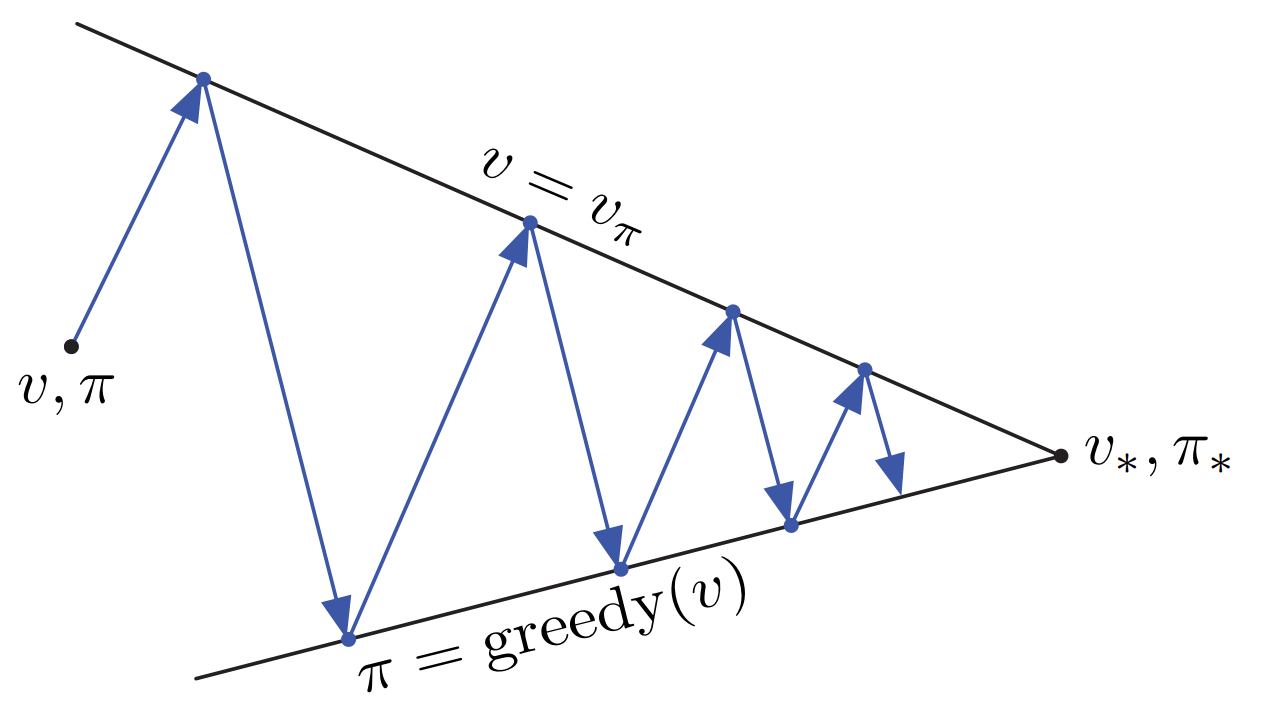
\includegraphics[width=\textwidth]{image/gpi2}
            \caption{Generalized Policy Iteration convergence.}
            \label{fig:gpi}
        \end{minipage}
    \end{figure}

    \subsection{Monte Carlo Methods}\label{subsec:monte-carlo-methods}
    \begin{wrapfigure}{r}{0.35\textwidth}
        \begin{center}
            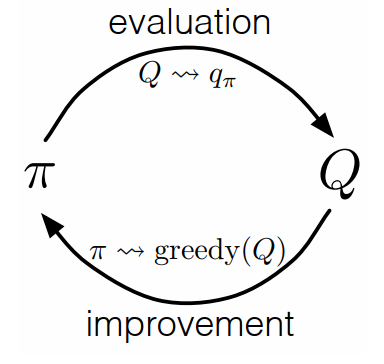
\includegraphics[width=0.33\textwidth]{image/mc-evaluation-improvement}
        \end{center}
    \end{wrapfigure}

    In this chapter, we explore Monte Carlo methods for estimating value functions in the context of reinforcement learning (RL) without assuming complete knowledge of the environment (\emph{transition probabilities} and \emph{reward function}). Monte Carlo methods use sample sequences of states, actions, and rewards from actual or simulated interactions with the environment for learning. These methods can be used to solve the RL problem for episodic tasks, where experience is divided into episodes and value estimates and policies are updated only on the completion of an episode.


    MC methods allow an agent to infer the optimal policy $\pi_*$ from the optimal action-value function $q_*(s,a)$ estimated through experience. MC methods use the iterative procedure Generalized Policy Iteration to incrementally infer $\pi_*$. First, a finite trajectory $(S_0,A_0,R_1,S_1,A_1,\cdots,R_n,S_n)$ is generated, where actions are selected according to a stochastic policy $\pi(a|s)$ and states and rewards come from the unknown environmental dynamics. From this episode, the return $G_t$ is computed for all state-action pairs reached. Then, the policy evaluation step is performed using the update equation~\cite{sutton2018reinforcement, FITMT25127, rao2022foundations}:

%    \begin{wrapfigure}[h!]
%        \includegraphics[width=\textwidth]
%        \caption{Monte Carlo convergence.}
%        \label{fig:mc}
%    \end{wrapfigure}

    \begin{equation}
        \label{eq:mc}
        q_{k+1}(s,a)=q_k(s,a)+\alpha(G_t-q_k(s,a))
    \end{equation}
    where $\alpha \in (0,1)$ is a learning rate and $G_t$ is the sum of discounted rewards starting from action $a$ in state $s$. The term $G_t - q_k(s, a)$ corrects the value of $q_{k+1}(s,a)$ in the direction of the target $G_t$. The index $k$ represents the current episode, and in the limiting case, $q_k(s,a) = q_{\pi}(s,a)$, where $\pi$ is the optimal policy~\cite{sutton2018reinforcement}.
    \begin{equation}
        \pi_0\xrightarrow{E}q_{\pi_0}\xrightarrow{I}
        \pi_1\xrightarrow{E}q_{\pi_1}\xrightarrow{I}
        \pi_2\xrightarrow{E}q_{\pi_2}\xrightarrow{I}
        \cdot
        \pi_*\xrightarrow{E}q_{\pi_*}
    \end{equation}

    Since MC methods do not require knowledge of the environment dynamics, a non-deterministic policy should be used for episode generation to ensure the exploration of all states and actions. A stochastic policy, such as the $\epsilon$-greedy approach, is commonly used in MC methods for exploration~\cite{FITMT25127}.

    \paragraph{Epsilon-Greedy Policy Exploration}
    The \textbf{$\epsilon$-greedy} approach for exploration selects actions randomly according to:
    \begin{equation}
        \pi'(a|S)=
        \begin{cases}
            1-\epsilon+\frac{\epsilon}{|\mathcal{A}|}&\text{if }a=A^*\\
            \frac{\epsilon}{|\mathcal{A}|}&\text{if }a\neq A^*
        \end{cases}
    \end{equation}
    where $A^*=\argmax_{a}(S_t, a)$. A Greedy action is an action with the highest estimated action value according to the current policy. The process of modifying action values in the policy evaluation step and setting a new policy in the policy improvement step is referred to as training the RL agent. It follows from \cref{eq:mc} that MC methods use the $G_t$ return of an episode, which can only be computed when the episode is completed. Therefore, MC methods can only be used in environments with finite, i.e. always ending, episodes. This strategy is called \emph{bootstrapping}, defined in \cref{subsubsec:n-step-bootstrapping}, when the methods do not need to wait for the end of the episode, but only need \emph{n-steps} to improve the policy, the whole strategy is called \emph{n-steps bootstrapping} and next method \emph{Temporal-Difference} uses this strategy to improve convergence to optimal value-function~cite{FITMT25127, sutton2018reinforcement, rl-course-david-silver}.

    \subsection{Temporal-Difference Methods}\label{subsec:temporal-difference-methods}

    Temporal-difference (TD) learning is a fundamental concept in reinforcement learning that combines ideas from Monte Carlo and dynamic programming (DP). TD methods allow for learning from raw experience without a model of the environment's dynamics, similar to Monte Carlo methods, but also update estimates based on other learned estimates, without waiting for a final outcome (like DP methods) using \emph{n-step bootstrapping}, defined in \cref{subsubsec:n-step-bootstrapping}. The relationship between TD, DP, and Monte Carlo is a recurring theme in reinforcement learning theory, and these ideas can be blended and combined in various ways. Both TD and Monte Carlo methods are used for policy evaluation, estimating the value function for a given policy. However, TD methods differ from Monte Carlo methods in that they update their value functions $v_{t+1}(s)$ or $q_{t+1}(a,s)$ estimates based on the non-terminal states observed in the experience, and they do not have to wait until the end of the episode to determine the increment to the value function~\cite{rl-course-david-silver, sutton2018reinforcement}.

    \subsubsection{n-step Bootstrapping}\label{subsubsec:n-step-bootstrapping}
    The n-step bootstrapping is a strategy to improve the convergence of the value function. The idea is to look only \emph{n-steps} ahead to update value function, instead of using the return of whole the episode. We show the difference in TD and MC methods.

    The \emph{TD target} is the sum of the reward and the discounted value of the next state, and it serves as the target for the TD update. The 1-step TD target $G_t$ is:
    \begin{equation}
        G_t=R_{t+1}+\gamma V(S_{t+1})
    \end{equation}
    or for 2-step TD target $G_t$:
    \begin{equation}
        G_t=R_{t+1}+\gamma R_{t+2}+\gamma^2V(S_{t+2})
    \end{equation}
    and for n-step TD target $G_t$:
    \begin{equation}
        G_t=R_{t+1}+\gamma R_{t+2}+\gamma^2R_{t+3}+\cdots+\gamma^{n-1}R_{t+n}+\gamma^nV(S_{t+n})
    \end{equation}
    while Monte Carlo Target $G_t$:
    \begin{equation}
        G_t=R_{t+1}+\gamma R_{t+2}+\gamma^2R_{t+3}+\cdots+\gamma^{T-t-1}R_{T}
    \end{equation}
%
%    \begin{figure}[h!]
%        \centering
%        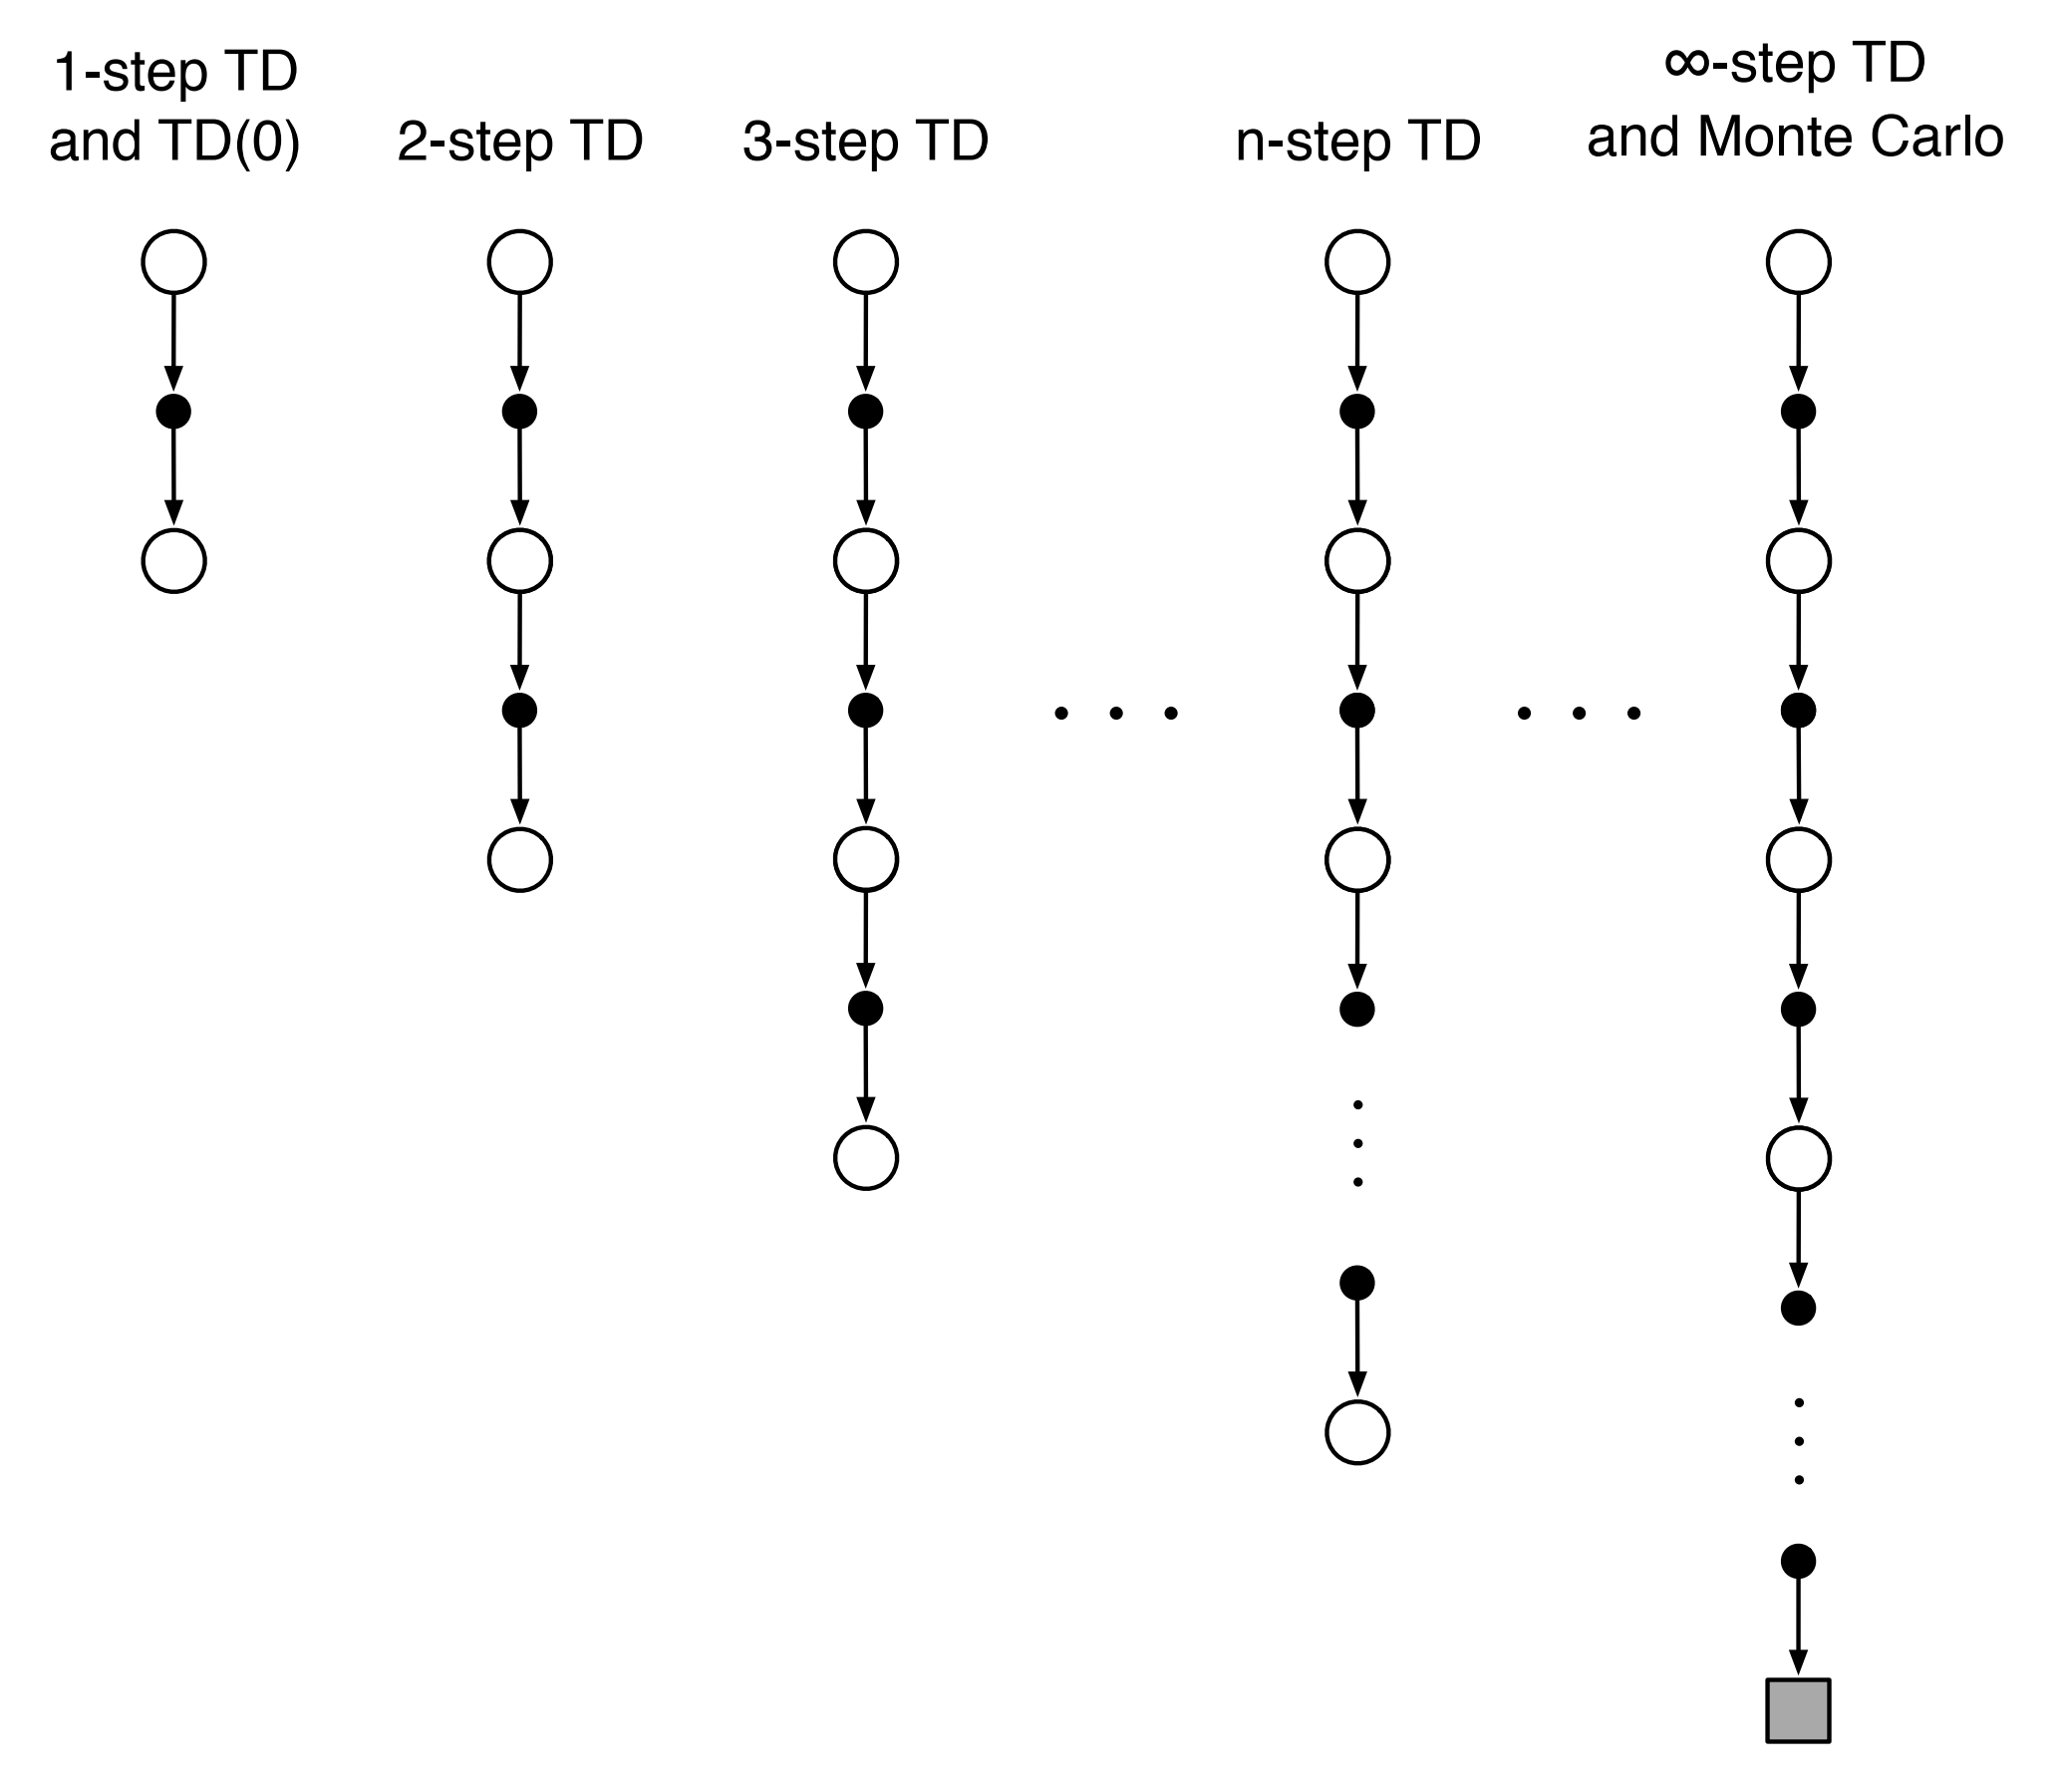
\includegraphics[width=0.7\textwidth]{image/n-step-bootstrapping}
%        \caption{The difference between TD and MC value function updates. The TD methods use the n-step bootstrapping to improve the convergence of the value function. While MC waits for the end of the episode to update the value function (the right-most sequence).}
%        \label{fig:n-step-bootstrapping}
%    \end{figure}

    The learning rule for (simplest) TD(0), also known as 1-step TD is the following update equation:
    \begin{equation}
        V(S_t)=V(S_t)+\alpha\cdot(R_{t+1}+\gamma\cdot V(S_{t+1})-V(S_t))
    \end{equation}
    where $ V(S_t) $ is the estimated value of state $ S_t $, $ \alpha $ is the learning rate, $ R_{t+1} $ is the reward received at time step $ t+1 $, $ \gamma $ is the discount factor, and $ V(S_{t+1}) $ is the current estimate of the value of the next state. On the other for the \emph{n-step bootstrapping} the learning rule for TD(n), also known as n-step TD is the following update equation:
    \begin{equation}
        V_{t:t+n}=R_{t+1}+\gamma R_{t+2}+\gamma^2R_{t+3}+\cdots+\gamma^{n-1}R_{t+n}+\gamma^nV(S_{t+n})\text{ , for }0\leq t\leq T
    \end{equation}

    The \emph{TD Error} is the difference between the TD target and the current value function estimate:
    \begin{equation}
        R_{t+1}+\gamma\cdot V(S_{t+1})-V(S_t)
    \end{equation}
    and represents the error in the current estimate of the value function, and the TD target represents the updated estimate of the value function for the current state. By using the TD error and TD target in the update rule, TD methods can learn from raw experience and update the value function at each time step, making them well-suited for online learning tasks~\cite{sutton2018reinforcement}.

%    The TD error at each time is the error in the estimate made at that time, depending on the next state and next reward. It is available at time $t + 1$, i.e., (t is the error in $V(S_t)$. If $V(s_t)$ does not change during the episode, then the Monte Carlo error can be written as a sum of \emph{TD errors}:
%    \begin{equation}
%        \begin{split}
%            G_t-V(S_t)&=R_{t+1}+\gamma G_{t+1}-V(S_t)+\gamma V(S_{t+1})-\gamma V(S_{t+1})\\
%            &=\delta_t+\gamma\delta_{t+1}+\gamma^2\delta_{t+2}+\ldots+\gamma^{T-t-1}\delta_{T-1}+\gamma^{T-t}\delta_T-V(S_T)\\
%            &=\delta_t+\gamma\delta_{t+1}+\gamma^2\delta_{t+2}+\ldots+\gamma^{T-t-1}\delta_{T-1}+\gamma^{T-t}(R_T+\gamma V(S_T)-V(S_T))\\
%            &=\sum_{k=t}^{T-1}\gamma^{k-t}\delta_k
%        \end{split}
%    \end{equation}


    In addition to TD(0), there are also other variations of TD methods such as TD($\lambda$), which is a family of methods that use eligibility traces to combine TD(0) updates with Monte Carlo-like updates. TD($\lambda$) methods have a parameter $\lambda$ that controls the trade-off between the bias and variance of the updates. When $\lambda$ is set to 0, TD($\lambda$) reduces to TD(0), and when $\lambda$ is set to 1, TD($\lambda$) reduces to Monte Carlo updates. TD($\lambda$) methods update the value function for not only the current state but also for all the states visited in the episode, weighted by their eligibility traces. The eligibility traces keeps track of the recent history of state visits and decays over time with a decay factor $\lambda$, which determines the credit assignment to different states~\cite{sutton2018reinforcement}.

    TD methods do not have to wait until the end of the episode to update the value function. Instead, they can make updates at each time step, using the observed reward and the estimate of the value function for the next state. This makes TD methods more computationally efficient and allows for online learning in environments where episodes are long or never-ending. Like DP and Monte Carlo methods, TD methods also use the iterative Generalized Policy Iteration (GPI) procedure to determine the optimal policy. The policy evaluation step in TD methods differs from Monte Carlo methods in that it uses the TD error, which is the difference between the TD target and the current estimate of the value function, as the update rule~\cite{sutton2018reinforcement}.

    \subsubsection{On-Policy Learning (SARSA)}\label{sec:td-sarsa}
    The TD methods use the action-value function for the evaluation step and iteratively determine $q_\pi(s,a)$. A TD method that implements this practice is called SARSA and adjusts the action-value function in the evaluation step for a state-action pair at each time-step of the episode as~\cite{sutton2018reinforcement, rl-course-david-silver}:
    \begin{equation}
        q_{t+1}(s,a)=q_t(s,a)+\alpha\left(R_{t+1}+\gamma q_t(s',a')-q_t(s,a)\right)
    \end{equation}

    The TD methods, such as SARSA, utilize the action-value function for evaluating and updating the action-value estimates. SARSA adjusts the action-value function at each time step of the episode based on the sequence of transitions $ (s, a, r, s', a') $ generated by the environment dynamics and the current epsilon-greedy policy. The updated action-value function is used to determine the new policy at the next time step. This process is repeated iteratively until optimal action value and policy functions are found. SARSA is an on-policy algorithm, as it evaluates and improves the same policy used for selecting actions~\cite{rl-course-david-silver}:
    \begin{equation}
        q_{t+1}(s,a)=q_t(s,a)+\alpha\left(R_{t+1}+\gamma\max_{a^*}q_t(s',a^*)-q_t(s,a)\right)
    \end{equation}

    \subsubsection{Off-Policy Learning (Q Learning)}\label{sec:td-q-learning}
    On the other hand, off-policy algorithms, like Q-learning, evaluate and improve one policy while using a different policy for selecting actions. This can be useful, for example, when introducing a new version of an agent with a different policy to learn from an old agent with a well-performing policy. In Q-learning, the action maximizing action ($ a^* $) of all action-value functions at a fixed state $ s' $ is always chosen when updating the action-value function for a given state-action pair $ (s, a) $, regardless of which action $ a^* $ of the policy was chosen. After updating the action-value function, the policy improvement step is performed using the epsilon-greedy approach with respect to the current policy ($ \pi $) and optionally the old policy ($ \mu $) as well. An off-policy TD control algorithm known as Q-learning, defined by~\cite{FITMT25127, sutton2018reinforcement}:
    \begin{equation}
        \label{eq:q-learning}
        Q(S_t,A_t)\leftarrow Q(S_t,A_t)+\alpha\left[R_{t+1}+\gamma\max_a Q(S_{t+1},a)-Q(S_t,A_t)\right]
    \end{equation}

    In this case, the learned action-value function, $Q$, directly approximates $q_*$, the optimal action-value function, independent of the policy being followed. This dramatically simplifies the analysis of the algorithm and enables early convergence proofs. The policy still has an effect in that it determines which state-action pairs are visited and updated. However, all that is required for correct convergence is that all pairs (transition matrix, example in \cref{fig:q-learning}) continue to be updated. This is a minimal requirement in the sense that any method guaranteed to find optimal behavior in the general case must require it. The Q-learning algorithm is show in \cref{alg:q_learning}~\cite{rl-course-david-silver, sutton2018reinforcement}.

    \begin{figure}[h!]
        \centering
        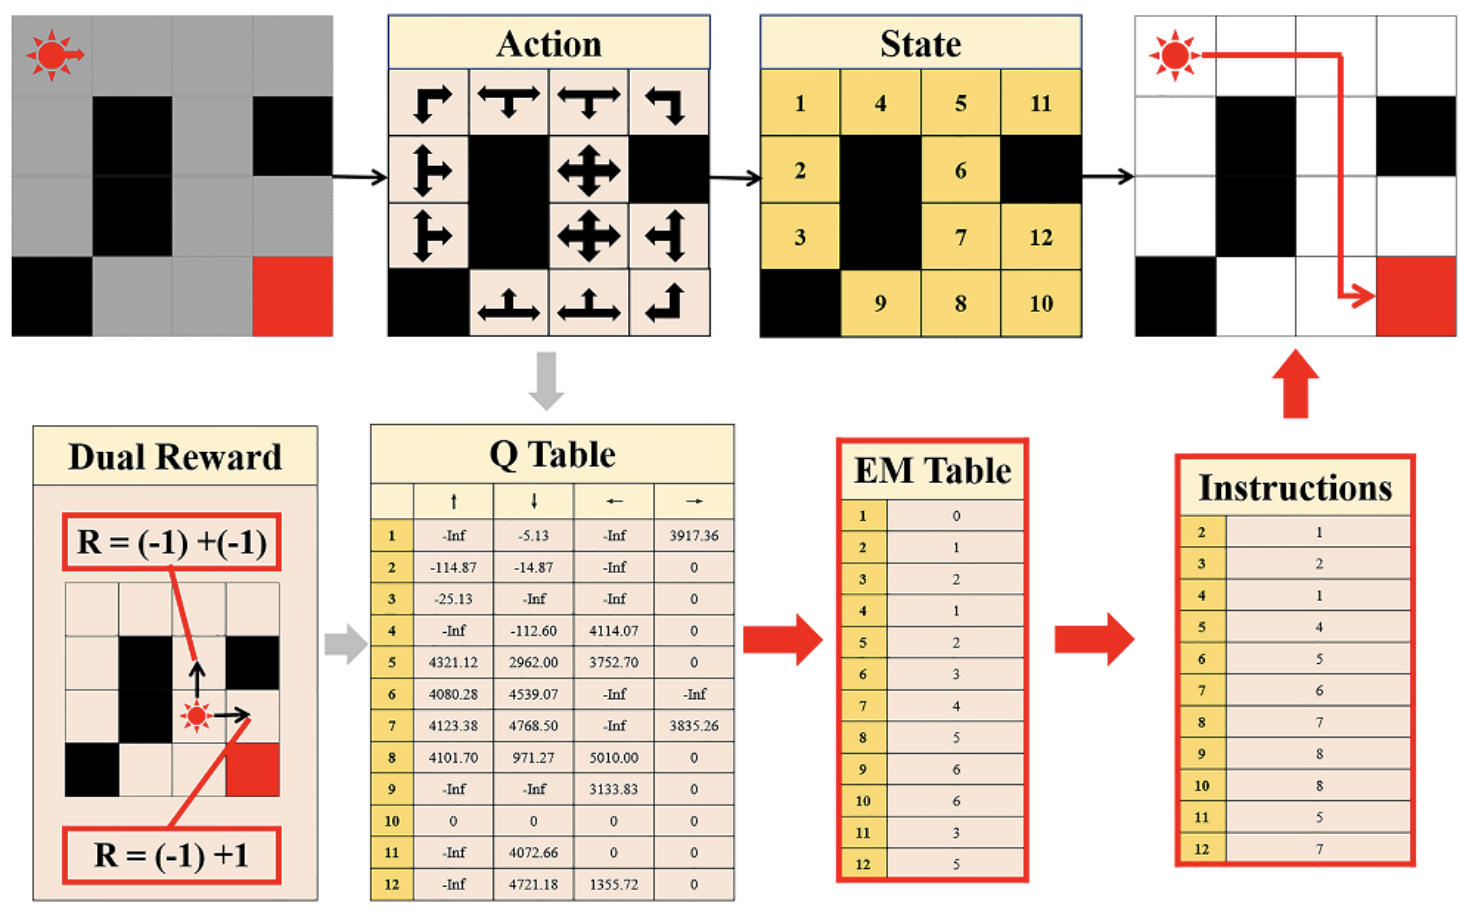
\includegraphics[width=0.9\textwidth]{image/q-learning}
        \caption{Q-learning table. How the training process updates the Q-table~\cite{article}.}
        \label{fig:q-learning}
    \end{figure}

    \subsection{Function Approximation}\label{subsec:function-approximation}
    The Monte Carlo and Temporal Difference algorithms discussed earlier are known as tabular methods because they rely on a matrix of action returns and values of dimension $|\mathcal{S}|\mathcal{A}|$. However, when the number of states or actions is extremely large, as in the case of \emph{Portfolio Allocation}, where the state space is the entire stock market, which may include data from thousands of stocks, the economic situation of the entire world, and the current political situation, all of these things need to be taken into account, so the state space is huge. The agent managing which assets it allocates funds to uses these observations, which very often change every single second, so this matrix becomes excessively huge. This poses a problem in terms of memory requirements, and it becomes almost impossible for an agent using MC or TD methods to comprehensively evaluate all the states and derive a policy~\cite{sutton2018reinforcement, FITMT25127}.

    Approximate Methods, which utilize parametrized function approximators such as decision trees, regression methods, or neural networks, differ from Tabular Methods in that they do not rely on matrices to estimate action-value returns. These methods have emerged as a solution approach to the limitations of Tabular Methods, as they are more memory efficient and capable of generalization. When neural networks are used as function approximators, then these algorithms are classified as Deep Reinforcement Learning (DRL)~\cite{FITMT25127}.

    The mean square error is defined as:
    \begin{equation}
        \overline{VE}(\bm{w})\doteq\sum_{s\in\mathcal{S}}\mu(s)\left[v_{\pi}(s)-\hat{v}(s,\bm{w})\right]
    \end{equation}

    where $\mu(s)$ is the probability of visiting state $s$, and $\hat{v}(s,\bm{w})$ is the output of the function approximator for state $s$ and weight vector $\bm{w}$.
    The objective is to minimize the error between the target output and the output of the function approximator, this is done by minimizing the $\overline{VE}(s)$.

    \subsubsection{Stochastic Gradient Descent}\label{subsubsec:stochastic-gradient-descent}
    Stochastic gradient descent (SGD) is a widely used method for function approximation in value prediction. It is well-suited for online reinforcement learning. In SGD, the weight vector is updated at each time step based on a small step in the direction of the negative gradient of the squared error for a single example. The step size is controlled by a positive parameter called the learning rate. The target output for each example may be a noisy approximation or a bootstrapping target~\cite{sutton2018reinforcement}.

    The Approximate Solution Methods use a \emph{function approximator} to approximate the action-value function $q_\pi(s,a)$ or the state-value function $v_\pi(s)$ as:
    $\hat{v}(s,\bm{w})\approx v_{\pi}(s)$ or $\hat{q}(s,a,\bm{w})\approx q_{\pi}(s,a)$, where $\bm{w}\in\mathbb{R}^d,d\in\mathbb{N}$

    The Gradient-descent update for state-value prediction is:
    \begin{equation}
        \label{eq:sgd}
        \bm{w}_{t+1}=\bm{w}_t-\alpha\left[v_\pi(S_t)-\hat{v}(S_t, \bm{w})\right]\nabla \hat{v}(S_t, \bm{w})
    \end{equation}
    where $\alpha$ is the learning rate, and $\nabla \hat{v}(S_t, \bm{w})$ is the gradient of the function approximator with respect to the weight vector $\bm{w}$.

    The \cref{eq:sgd} can be extended to n-step returns:
    \begin{equation}
        \begin{split}
            \bm{w}_{t+n}\doteq\bm{w}_{t+n-1}+\alpha\left[G_{t:t+n}-\hat{v}(S_t,\bm{w}_{t+n-1})\right]\nabla\hat{v}(S_t,\bm{w}_{t+n-1})
        \end{split}
    \end{equation}
    where the n-step return is:
    \begin{equation}
        \begin{split}
            G_{t:t+n}\doteq R_{t+1}+\gamma R_{t+2}+\dots+\gamma^{n-1}R_{t+n}+\gamma^n\hat{v}(S_{t+n},\bm{w}_{t+n-1})
        \end{split}
    \end{equation}

    On the other hand the Gradient-descent update for action-value prediction is:
    \begin{equation}
        \bm{w}_{t+1}=\bm{w}_t+\alpha \left[U_t-\hat{q}(S_t,A_t,\bm{w}_t)\right]\nabla \hat{q}(S_t,A_t,\bm{w}_t)
    \end{equation}
    where the $U_t$ is the TD target, as mentioned earlier, and the $\nabla \hat{q}(S_t,A_t,\bm{w}_t)$ is the gradient of the function approximator with respect to the weight vector $\bm{w}$~\cite{sutton2018reinforcement}.

    The weights for one-step SARSA are updated using the following rule:
    \begin{equation}
        \bm{w}_{t+1}=\bm{w}_t+\alpha\left[R_{t+1}+\gamma q_{\pi}(S_{t+1},A_{t+1},\bm{w})-q_{\pi}(S_t,A_t,\bm{w})\right]\nabla q_{\pi}(S_t,A_t,\bm{w})
    \end{equation}
    and can be extended to \emph{n-step SARSA}:
    \begin{equation}
        \bm{w}_{t+1}=\bm{w}_t+\alpha\left[G_{t:t+n}-\hat{q}_{\pi}(S_t,A_t,\bm{w})\right]\nabla\hat{q}_{\pi}(S_t,A_t,\bm{w})
    \end{equation}


    The update is performed in a way that each vector's component responsible for a part of the error is updated accordingly, with a higher share of the error being adjusted if the slope of the error with respect to that component is large. The weights are adjusted until the difference between two subsequent updates is less than a defined $\varepsilon$ value (typically a small number), at which point $q_{\pi}$ is considered found and the optimal policy can be derived. In practice, early stopping is often used in deep learning instead of $\varepsilon$. Now that the vectors of state-action values are no longer represented as a look-up table, they can be written as an approximation by the neural network. Furthermore, the policy improvement step can also incorporate the $\epsilon$-greedy approach for action selection~\cite{FITMT25127, rao2022foundations, rao2022foundations}.

    \begin{equation}
        \bm{\hat{y}} = \begin{pmatrix}
                           \hat{q}(s,\textcolor[RGB]{50,150,50}{a_1},\bm{w}) \\
                           \textcolor[RGB]{50,150,50}{\vdots}                \\
                           \hat{q}(s,\textcolor[RGB]{50,150,50}{a_n},\bm{w})
        \end{pmatrix}
    \end{equation}


    \section{Policy-based learning}\label{sec:policy-based}
    In this section, we explore a new approach that involves learning a parameterized policy without relying on action-value estimates. The policy's parameter vector is denoted as $\bm{\theta}$, and the probability of selecting actions is represented as $\pi(a|s, \bm{\theta})$. We focus on methods that update the policy parameter based on the gradient of a scalar performance measure $J(\bm{\theta})$, aiming to maximize performance without necessarily using a value function for action selection. But later, in \cref{subsec:actor-critic-policy-gradient-methods} we will describe \emph{Actor-Critic} methods that combine the policy gradient methods with the value-based methods~\cite{sutton2018reinforcement}.

    \subsection{Stochastic Policy Gradient Methods}\label{subsec:policy-gradient}
    All algorithms that use a parameterized policy are referred to as policy gradient methods. We can represent the policy with a parameter vector $ \bm{\theta} \in \mathbb{R}^d $, where $ d \in \mathbb{N} $. Then, extending \cref{eq:policy}, we can formulate the probability of executing action $ a $ in state $ s $ with parameters $ \bm{\theta} $ at time-step $ t $ of policy $ \pi_{\bm{\theta}} $ as:
    \begin{equation}
        \pi(a|s,\bm{\theta})=Pr\left[A_t=a|S_t=s,\bm{\theta}_t=\bm{\theta}\right]
    \end{equation}

    If a performance measure $ J(\bm{\theta}) $ is introduced on the parameter vector, then the policy gradient methods can iteratively update the parameter vector using the gradient ascent procedure as follows:
    \begin{equation}
        \bm{\theta}_{t+1}=\bm{\theta}_t+\alpha\widehat{\nabla J(\bm{\theta}_t)}
    \end{equation}
    where $\widehat{\nabla J(\bm{\theta}_t)}$ is a stochastic estimate whose expectation is the true gradient of $ J(\bm{\theta}) $ concerning $ \bm{\theta} $.

    Deriving a loss function for the performance measure in policy gradient methods is not as straightforward as in the case of value-based methods. Similar to the distinction between MC methods and TD methods, we need to differentiate between finite and infinite episodes. For both cases, the theorem on policy gradients provides a way to compute the gradient $ \nabla J(\bm{\theta}) $~\cite{sutton2018reinforcement, FITMT25127}.

    \subsubsection{The Policy Gradient Theorem}\label{subsubsec:policy-gradient-theorem}
    For finite episodes, we can measure the quality of the parameter vector based on the return of the first state of the episode. The policy gradient theorem for the episodic case establishes the gradient of the return of the first state of the episode with respect to the parameter vector.

    First note that the gradient of the state-value function can be
    written in terms of the action-value function as~\cite{sutton2018reinforcement}:


    \begin{equation}
        \begin{split}
            \nabla v_{\pi_{\bm{\theta}}}(s)&=\nabla\left(\sum_{a}\pi(a|s,\bm{\theta})q_{\pi_{\bm{\theta}}}(s,a)\right)\\
            &=\sum_{a}(\nabla\pi(a|s,\bm{\theta})q_{\pi_{\bm{\theta}}}(s,a)+\pi(a|s,\bm{\bm{\theta}})\nabla q_{\pi_{\bm{\theta}}}(s,a))\\
            &\mspace{10mu}\vdots\\
            &=\sum_{s}\sum_{k=0}^{\infty}Pr(s\rightarrow x,k,\pi_{\bm{\theta}})\sum_{a}\nabla\pi(a|s,\bm{\theta})q_{\pi_\theta}(s,a)
        \end{split}
    \end{equation}
    where $Pr\left[s \rightarrow x, k, \pi_{\bm{\theta}}\right]$ is the probability of a state transition from $s$ to $x$ in $k$ steps under policy $\pi(a | s, \bm{\theta})$. This probability thus serves as a weighting of the gradient of the return. Moreover, this can be further written:

    \begin{equation}
        \label{eq:policy_gradient}
        \begin{split}
            \nabla J(\bm{\theta})&=\nabla v_{\pi_{\bm{\theta}}}(s_0)\\
            &=\sum_{s}\left(\sum_{k=0}^{\infty}Pr(s_0\rightarrow s,k,\pi_{\bm{\theta}})\right)\sum_{a}\nabla\pi(a|s,\bm{\theta})q_{\pi_{\bm{\theta}}}(s,a)\\
            &=\sum_{s}\eta(s)\sum_{a}\nabla\pi(a|s,\bm{\theta})q_{\pi_{\bm{\theta}}}(s,a)\\
            &=\sum{s'}\eta(s')\sum_{s}\frac{\eta(s)}{\sum_{'s}\eta(s')}\sum{a}\nabla\pi(a|s,\bm{\theta})q_{\pi_{\bm{\theta}}}(s,a)\\
            &=\sum_{s'}\eta(s')\sum_{s}\mu(s)\sum_{a}\nabla\pi(a|s,\bm{\theta})q_{\pi_{\bm{\theta}}}(s,a)\\
            &\propto\sum_{s}\mu(s)\sum_{a}\nabla\pi(a|s,\bm{\theta})q_{\pi_{\bm{\theta}}}(s,a)\\
        \end{split}
    \end{equation}
    where $s_0$ is the first state of the episode, $s'$ is the next state, $\eta(s)$ is the probability of being in state $s$ at particular time-step and $G_t$ is the return of the episode~\cite{sutton2018reinforcement, FITMT25127}.

    The \cref{eq:policy_gradient} shows, that $J(\bm{\theta})$ is proportional to the probability sum of $\sum_s \mu(s)$, which denotes the likelihood that the agent is in the state $s$, multiplied by the sum of weighted gradients of the probabilities for the selection of actions. The proportionality constant is represented as $\sum_s \eta(s)$. Practically, this equation provides insight that when the agent is in a state, it should move in the direction of weights that represent the greatest increase in the probability of selecting an action in that state, weighted by the expected return for that state and action~\cite{FITMT25127}.

    In the case of infinite episodes, the performance measure $J(\bm{\theta})$ is the average reward per time-step. The gradient $\nabla J(\bm{\theta})$ can then be determined by the theorem of policy gradients for infinite episodes, see \cref{eq:policy_gradient_infinite}, thus the calculations of the gradient for the infinite case correspond to those of the episodic case.
    \begin{equation}
        \label{eq:policy_gradient_infinite}
        \nabla J(\bm{\theta})=\sum_s\mu(s)\sum_a\nabla\pi(a|s,\bm{\theta})q_{\pi_\theta})(s,a)
    \end{equation}

    \subsubsection{Discrete Action Space}
    Policy gradient methods allow for flexible parameterization of the policy as long as it is differentiable with respect to its parameters. A common approach for discrete action spaces is to use softmax in action preferences, where actions with higher preferences have higher probabilities of being selected:
    \begin{equation}
        \label{eq:softmax}
        \pi(a|s, \bm{\theta}) = \frac{e^{h(s,a,\bm{\theta})}}{\sum_b e^{h(s,b,\bm{\theta})}} ,
    \end{equation}
    where $\pi(a|s, \theta)$ is the probability of selecting action $a$ in state $s$ with policy parameterized by $\theta$, and $h(s,a,\theta)$ is the parameterized numerical preference for state-action pair $(s,a)$. The preferences $h(s,a,\theta)$ can be parameterized using deep neural networks or linear features:
    \begin{equation}
        \label{eq:softmax_linear}
        h(s,a,\bm{\theta}) = \bm{\theta}^T x(s,a) ,
    \end{equation}
    where $\theta$ is the vector of parameters (e.g., connection weights) and $x(s,a)$ is a feature vector for state-action pair $(s,a)$. Choosing an appropriate reduction schedule for the temperature parameter in softmax can be challenging without prior knowledge of the true action values~\cite{sutton2018reinforcement}.

    \subsection{REINFORCE: Monte Carlo Policy Gradient}\label{subsec:monte-carlo-policy-gradient-methods}
    The REINFORCE algorithm is a purely policy-based approach that utilizes the return of complete finite episodes for parameter updates, that is the reason of \emph{Monte Carlo} in the name of this method. Similar to classical TD methods, it adjusts the return gradually with each time step, unlike MC methods where the return is updated at the end of each episode~\cite{rl-course-david-silver, sutton2018reinforcement}.

    Firts we extend the introduction of $A_t$ in REINFORCE similar to how we introduced $S_t$ in \cref{eq:policy_gradient}, by replacing a sum with an expectation under the policy $\pi$, and then sampling from it. We add the necessary weighting by multiplying and dividing the summed terms by $\pi(a|S_t, \bm{\theta})$ without changing the equality. Continuing from \cref{eq:policy_gradient}, we have~\cite{sutton2018reinforcement, rl-course-david-silver}:

    \begin{equation}
        \label{eq:policy_gradient_2}
        \begin{split}
            \nabla J(\bm{\theta})&\propto E_{\pi}\left[\sum_{a}q_{\pi_{\bm{\theta}}}(s,a)\nabla\pi(a|s,\bm{\theta})\right]\\
            &=E_{\pi}\left[\sum_{a}\pi(a|s,\bm{\theta})q_{\pi_{\bm{\theta}}}(s,a)\frac{\nabla\pi(a|s,\bm{\theta})}{\pi(a|s,\bm{\theta})}\right]\\
            &=E_{\pi}\left[\sum_{a}\pi(a|s,\bm{\theta})q_{\pi_{\bm{\theta}}}(s,a)\nabla\log\pi(a|s,\bm{\theta})\right]\\
            &=E_{\pi}\left[\sum_{a}G_t\nabla\log\pi(a|s,\bm{\theta})\right]
        \end{split}
    \end{equation}

    In this algorithm, the weight vector $\bm{\theta}$ is updated using the product of the return $G_t$ and the gradient vector $\nabla \ln \pi(a | s, \bm{\theta})$, which represents the steepest increase in the probability of selecting action $a$ in state $s$. This policy parameterization vector adjustment ensures that $\bm{\theta}$ is updated with the scaling factor $G_t$. Update equation for the policy parameterization vector $\bm{\theta}$ is~\cite{FITMT25127, sutton2018reinforcement, rl-course-david-silver}:
    \begin{equation}
        \begin{split}
            \bm{\theta}_{t+1}&\doteq\bm{\theta}_{t}+\alpha G_t \frac{\nabla\pi(a|s,\bm{\theta}_t)}{\pi(a,s,\bm{\theta}_t)}\\
            \bm{\theta}_{t+1}&\doteq\bm{\theta}_{t}+\alpha G_t \nabla\ln\pi(a|s,\bm{\theta}_t)
        \end{split}
    \end{equation}
    and the final equation used in the algorithm looks like this (including discount factor):
    \begin{equation}
        \begin{split}
            \bm{\theta}_{t+1}&\doteq\bm{\theta}_{t}+\alpha\gamma^t G_t \nabla\ln\pi(a|s,\bm{\theta}_t)
        \end{split}
        \label{eq:REINFORCE}
    \end{equation}

    The algorithm employs stochastic gradient ascent for optimization, as the weights are updated at each time step. Depending on whether the action space of the environment is discrete or continuous, the policy parametrizations described in the previous subsection can be used for the gradient $\nabla\ln\pi(a|s,\bm{\theta}_t)$. One drawback of this algorithm is the high variability in returns between time steps and the associated "slowness" of the learning process. This variance arises from the non-adaptive and loose formulation of the scaling factor. See \cref{alg:REINFORCE} for the pseudocode of the REINFORCE algorithm.

    The improvement of the REINFORCE algorithm is the REINFORCE with Baseline $b(s)$.

    \begin{equation}
        \nabla J(\bm{\theta})\propto E_{\pi}\left[\sum_{a}(q_\pi(s,a)-b(s))\nabla\log\pi(a|s,\bm{\theta})\right]
    \end{equation}

    \begin{equation}
        \begin{split}
            \bm{\theta}_{t+1}&\doteq\bm{\theta}_{t}+\alpha\gamma^t (G_t-b(s)) \nabla\ln\pi(a|s,\bm{\theta}_t)
        \end{split}
        \label{eq:REINFORCE_with_baseline}
    \end{equation}

    One natural choice for the baseline is an estimate of the state value, $\hat{v}(S_t, w)$, where $w \in \mathbb{R}^d$ is a weight vector learned by one of the methods presented in previous sections~\cite{FITMT25127, sutton2018reinforcement, rl-course-david-silver}. The reason why we introduce REINFORCE with Baseline is that the next \cref{subsec:actor-critic-policy-gradient-methods} will introduce Actor-Critic methods, which are a combination of REINFORCE with Baseline and TD methods.

    \subsection{Actor-Critic Policy Gradient Methods}\label{subsec:actor-critic-policy-gradient-methods}
    In actor-critic methods, the state-value function is used to assess actions, including the second state of a transition, and estimate the one-step return. This is different from REINFORCE with baseline, which only estimates the value of the first state. One-step actor-critic methods are fully online and incremental, making them easier to understand and implement compared to eligibility trace methods. A vector of constants can be used as the baseline. The concept of Actor-Critic methods can be formulated, when a function approximator with bootstrapping, such as TD(0) or SARSA(0), is used as the baseline. In this case, the Critic computes the scaling factor and the Actor adjusts the policy parameter $\bm{\theta}$. The weight update formula for the Actor-network is then as follows~\cite{sutton2018reinforcement, FITMT25127}:
    \begin{equation}
        \begin{split}
            \theta_{t+1}&\doteq\theta_t\alpha\left(G_{t:t+1}-\hat{v}(S_t,\bm{w})\right)\nabla\ln\pi(A_t|S_t,\theta_t)\\
            &=\theta_t+\alpha\left(R_{t+1}+\gamma\hat{v}(S_{t+1},\bm{w}-\hat{v}(S_t,\bm{w}))\right)\nabla\ln\pi(A_t|S_t,\theta_t)\\
            &=\theta_t+\alpha\delta_t\nabla\ln\pi(A_t|S_t,\theta_t)
        \end{split}
    \end{equation}

    The policy gradient update formula can be written as:
    \begin{equation}
        \nabla J(\bm{\theta})\propto\sum\mu(s)\sum(q_\pi(\bm{\theta})(s,a)-b(s))\nabla\pi(a|s,\bm{\theta})
    \end{equation}

    \subsubsection{Continuous Action Space}
    Continuous Action-space Policy Gradient methods can be used in environments with discrete as well as with continuous action space. Value-based methods have the disadvantage that they can only be used in environments with discrete action space. Whether a given policy gradient method can be used on discrete or continuous action space is determined by the policy parametrization. In the case of a discrete action space, a numerical value function, denoted as $ h(s, a, \theta) \in \mathbb{R} $, can be computed for each state-action pair. The computation of these values can be done, for example, via a neural network. An exponential Softmax distribution can then specify the probability with which an action should be selected, as shown in \cref{eq:softmax}~\cite{FITMT25127, sutton2018reinforcement}:

    For large or continuous action spaces, instead of evaluating individual actions, parameters of distribution functions such as the Normal distribution are computed. The parameters of the Normal distribution are the mean $\mu\in\mathbb{R} $ and the variance $ \sigma^2\leq 0$. The Normal distribution is defined on $\mathbb{R}$, which makes it suitable for continuous action spaces. The mean and variance can be parametrized and approximated as~\cite{sutton2018reinforcement}:

    \begin{equation}
        \label{eq:normal_distribution_policy}
        \pi(a | s, \theta) = \frac{1}{\sqrt{2\pi} \sigma(s, \theta)} \exp\left(-\frac{(a - \mu(s, \theta))^2}{2\sigma(s, \theta)^2}\right) \tag{2.37}
    \end{equation}

    From \cref{eq:normal_distribution_policy}, it can be seen that the policy parameter vector can be described as $ \theta = (\theta_{\mu}, \theta_{\sigma}) $, and its parameters can be computed using a single neural network. This enables the implementation of continuous actions for stochastic policies~\cite{FITMT25127, sutton2018reinforcement, rl-course-david-silver}.


%    \section{RL algorithms}
%    TODO
%
%    \subsection{Asynchronous Actor Critic}
%    TODO
%
%    \subsection{Deep Deterministic Policy Gradient}
%    TODO
%
%    \subsection{Deep Q Network}
%    TODO
%
%    \subsection{Proximal Policy Optimization}
%    TODO
%
%    \subsection{Soft Actor Critic}
%    TODO
%
%    \subsection{Twin Delayed DDPG}
%    TODO
%
%
%    \section{Model-based}\label{sec:model-based}
%    As mentioned in Section~\cref{sec:rl-introduction}, RL algorithms can be broadly categorized into two main types: model-free and model-based. Model-based methods rely on \emph{planning} as their primary component, while model-free methods rely on \emph{learning}~\cite{sutton2018reinforcement}. Despite their distinctions, both approaches involve computing value functions and using them to update approximate value functions based on future events.
%
%    One popular approach is to use a probabilistic model of the environment, which can be represented as a transition function $P(s_{t+1}|s_t, a_t)$ that describes the probability of transitioning from state $s_t$ to state $s_{t+1}$ when taking action $a_t$. Some popular probabilistic model-based RL methods include Monte Carlo Tree Search, Neural Network Dynamics, and Probabilistic Ensembles with Trajectory Sampling.
%
%    Another approach in model-based RL is to use a learned deterministic model of the environment, which can be represented as a function $f(s_t, a_t)$ that directly maps states and actions to the next states. Deterministic model-based RL methods, such as World Models, learn an encoder to represent states, a recurrent neural network (RNN) to model dynamics, and a decoder to generate predicted next states.
%
%    \subsection{Planning}\label{subsec:planning}
%    A model of the environment refers to anything that an agent can use to predict the outcome of its actions. It can be either stochastic, where there are multiple possible outcomes with associated probabilities, or deterministic, where the outcome is fixed. Distribution models provide a description of all possible outcomes and their probabilities, while sample models generate a single outcome sampled from the probabilities.
%
%    Planning, in the context of artificial intelligence, refers to a computational process that takes a model of the environment as input and produces or improves a policy for interacting with the environment. There are two main approaches to planning: \emph{state-space} planning and \emph{plan-space} planning. In \emph{state-space} planning, the focus is on searching through the \textbf{space of states} to find an optimal policy or path to a goal. Value functions are computed over states to guide the search. On the other hand, in \emph{plan-space} planning, the search is conducted through the \textbf{space of plans}, where operators transform one plan into another, and value functions, if any, are defined over the space of plans. Plan-space methods are challenging to efficiently apply to the stochastic sequential decision problems that are the primary focus in reinforcement learning~\cite{sutton2018reinforcement}.
%
%    The common structure in \emph{state-space} planning and learning methods, as presented in this chapter, is that value functions are computed as intermediate steps using simulated experience. Value functions are used to estimate the expected future rewards of different actions or states, and they play a key role in improving the policy of an agent. A simulated experience is generated by using the model to simulate the environment, and the agent can update its value functions based on this simulated experience to guide its decision-making process.
%
%    \begin{center}
%        \begin{tikzpicture}[auto]
%% Nodes
%            \node[] (s) {model};
%            \node[right=1cm of s] (a) {simulated experience};
%            \node[right=2cm of a] (r) {values};
%            \node[right=1cm of r] (s_p) {policy};
%
%% Arrows
%            \draw[thick, ->] (s) -- (a);
%            \draw[thick, ->] (a) -- (r) node[midway, anchor=south] {backups};
%            \draw[thick, ->] (r) -- (s_p);
%        \end{tikzpicture}
%    \end{center}
%
%    Dynamic programming methods fit the structure of making sweeps through the space of states, generating possible transitions, computing backed-up values, and updating state estimates. Other state-space planning methods also fit this structure, with differences in updates, order, and retention of backed-up information. Planning methods are related to learning methods in estimating value functions through backing-up operations. Learning methods use real experience from the environment, while planning uses simulated experience from a model. Ideas and algorithms can be transferred between planning and learning. Planning in small, incremental steps allows for efficient interruption and redirection, which is beneficial for intermixing planning with acting and learning the model. Planning in small steps may be the most efficient approach for large planning problems~\cite{sutton2018reinforcement}.
%
%    See \cref{alg:random-sample-one-step-tabular-q-planning}
%
%    \subsection{Dyna-Q}\label{sec:dyna-q}
%    Dyna-Q includes all of the processes shown in the \cref{fig:dyna-q-learning}: planning, acting, model-learning, and direct RL—all occurring continually. The Dyna-Q algorithm is a learning method that combines both planning and direct RL approaches (MC and TD). Planning involves optimizing strategies through simulations using a learned environment model, while direct RL focuses on improving the value and policy functions using real experiences from interactions with the environment, as depicted in \cref{fig:dyna-q-learning}. The Dyna agent interacts with the real environment to collect empirical data and iteratively improves its policy using \cref{eq:q-learning}. At the same time, an environment model is learned using real experiences, and simulation data generated by the model are used to update the action-value function using the Q-Learning update method.
%
%    In tasks such as path planning, obtaining real experiences from interactions with the environment can be costly and time-consuming. However, using the learned environment model to generate simulation experiences is faster and more convenient, which can reduce the training time of the algorithm. See the~\cref{alg:dyna-q}.
%
%    \begin{figure}
%        \centering
%        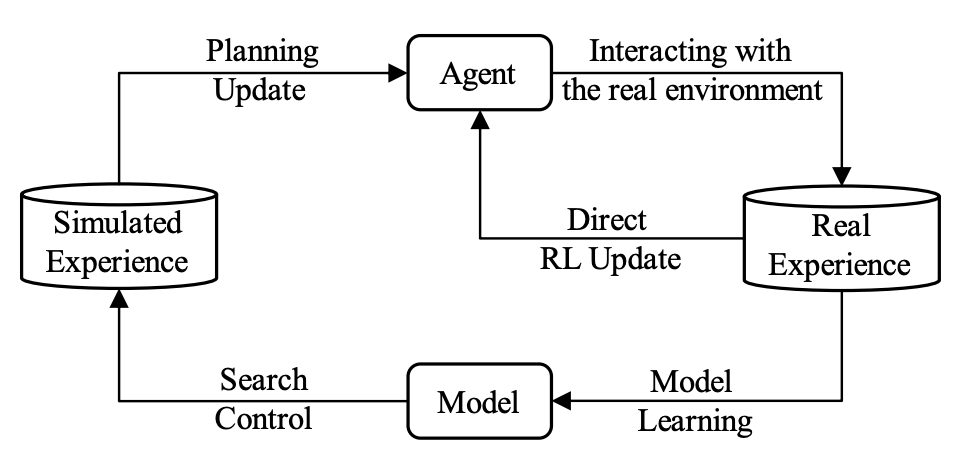
\includegraphics[width=0.5\textwidth]{image/dyna-q-learning}
%        \caption{Dyna-Q learning process.}
%        \label{fig:dyna-q-learning}
%    \end{figure}
%
%    \subsection{Trajectory Sampling}\label{subsec:trajectory-sampling}
%
%    \subsection{Summary}\label{subsec:summary}
%
%    Model-based RL offers several advantages over model-free methods. One major advantage is sample efficiency, as the agent can use the learned model of the environment to plan and generate simulated trajectories for learning, reducing the need for costly real-world interactions. Additionally, model-based RL can enable the agent to handle complex, high-dimensional state spaces and long-horizon tasks more effectively.
%
%    However, model-based RL also faces challenges. One challenge is the accuracy of the learned model, as any errors in the model can lead to suboptimal policies. Another challenge is the computational cost of planning and decision-making using the learned model, as it requires additional computation compared to direct action selection in model-free methods.
%
%    In conclusion, model-based RL is a promising approach that can offer sample-efficient learning and improved performance in complex environments. Various methods, such as probabilistic models and deterministic models, have been proposed in the literature. Despite some challenges, model-based RL continues to be an active area of research in machine learning.
%
%
%    \section{Exploration vs. Exploitation}\label{sec:exploration-vs-exploitation}
%
%    \subsection{Greedy}\label{subsec:greedy}
%
%    \subsection{Epsilon-Greedy}\label{subsec:epsilon-greedy}
%
%    \subsection{Upper Confidence Bound}\label{subsec:upper-confidence-bound}


\end{document}
